%%%%%%%%%%%%%%%%%%%%%%%%%%%%%%%%%%%%%%%%%%%%%%%%%%%%%%%%%%%%%%%%%%%%%%%%%%%%%%%%
% object_id_reco_corr: Select of showering and tracking events:
%%%%%%%%%%%%%%%%%%%%%%%%%%%%%%%%%%%%%%%%%%%%%%%%%%%%%%%%%%%%%%%%%%%%%%%%%%%%%%%%
\chapter{Object Identification and Triggers  }
\label{ch:objs}
This chapter focuses on the definitions and identifications of objects used in this analysis. While the previous chapter focuses on defining the backgrounds and signal region studied in this analysis, the focus here is on the details of implementing this search in the physical \CMS detector. Selecting events and reconstructing particles in real data, and comparing them to simulated events, pose many unique challenges. Covered in this chapter will be the trigger criteria used to select events for saving to disk at \CMS, and the reconstruction, identification, and correction of jet, muon and electron objects used in this analysis. The process of creating these objects, called Particle Flow, is discussed in Section~\ref{sec:particle_flow}.

\section{Jets}

\subsection{Jet Reconstruction}
\label{sec:jetreco}

In the boosted analysis, a larger jet is used (AK8), with \ensuremath{R=0.8}, and in the resolved analysis, a smaller jet is used (AK4), with \ensuremath{R=0.4}. After the jet has been constructed with PF particles, additional algorithms are used in an attempt to reduce the effects of pileup. For the AK8 jets, the pileup per particle identification (PUPPI) algorithm is used \cite{PUPPI}.  This weights each PF particle prior to being clustered in the jet based on a calculated probability of it coming from a pileup vertex.  This is done based on several parameters, event pileup properties, local energy distribution, and tracking.  The AK4 jets use charged hadron subtraction (CHS) where all charged hadrons which are not identified as coming from the primary vertex are removed from the jet.
\subsection{Identification}
This analysis uses the official recommended requirements for jet quality from the \CMS JetMET group. The identification is designed to reject low quality jets. Jets that are not of interest to this analysis can be produced by in various ways including: the overlap of multiple pileup particles, anomolous noise in subdetectors and non-hadronic lepton seeding. The jet quality requirements significantly reduce the presence of these jets in our selection.  For the resolved analysis, we additionally veto jets which may be created by an energetic lepton and random PF particles around it.
For AK4 jets the following requirements are used:
\begin{description}
  \begin{itemize}
      %\item there is at least one constituent in the jet,
      \item the neutral and charged electromagnetic energy fractions must be less than 90\%,
      \item the neutral hadronic energy fraction must be less than 90\% (2016) or 80\% (2017,2018),
      \item there is at least one charged hadron in the jet and the charged, hadronic energy fraction is greater than 0\%,
      \item the muon energy fraction must be less than 80\%.
  \end{itemize}
\end{description}
For AK8 jets, largely the same requirements are used, but there is no veto on a jet seeded by a lepton. This increases our efficiency, as an energetic lepton is already required to be in the jet, and these requirements could conflict. The AK8 jet requirements are:
\begin{description}
  \begin{itemize}
      %\item there is at least one constituent in the jet,
      \item the neutral and charged electromagnetic energy fractions must be less than 99\% (for 2016),
      \item the neutral hadronic energy fraction must be less than 90\%,
      \item there is at least one charged hadron in the jet and the charged, hadronic energy fraction is greater than 0\%.
  \end{itemize}
\end{description}

All AK8 and AK4 jets considered in the analysis must pass these identification requirements. With a quality selection of jets in each event, kinematic requirements can be placed on the jets to identify signal and background events as detailed in Chapter~\ref{ch:strategy}.

\subsection{Corrections}
The differences between the jet energy in simulation and data requires additional correction. These corrections are produced by a group within \CMS which studies the performance of jet objects in the detector. Typically, the energy corrections are $2-3\%$.
%L2, and L3 corrections are applied to account for detector non-linearities.  
%Some of the differences between the data and simulation of jets are corrected studying the \pt balance in \ensuremath{\gamma}+jets and Z+jets events.  
Jet energies in data and simulation differ by a scale-factor dependent on the \pt and $\eta$ of the jets. The resolution of the jet energies are additionally different in simulation and data.  As such, a per-jet random smearing is in applied to simulated jets to adjust their resolutions into agreement with data. 

The boosted analysis relies on a somewhat unique jet finding configuration, as the heavy neutrino is reconstructed as an AK8 jet as part of this analysis. Jet energy corrections are studied and calculated using a simulated QCD sample.  The generated right-handed neutrino energy was compared to the energy of the AK8 jet reconstructed from it, both with and without jet energy corrections applied.  This is shown in Fig.~\ref{fig:jetEvsNRE}.  It can be seen that the corrections have a minimal effect on the energy.  The peak is in substantially the same place, and the relative broadness of the reconstructed energy is expected.  The study and corrections applied are based on the 2016 detector conditions, but no significant changes were expected for 2017 and 2018 data, and they were not studied. Additionally, jet corrections can be correlated between years, and this is discussed further in Section~\ref{sec:multiyearsys}.

\begin{figure}[!tp]
    \centering
    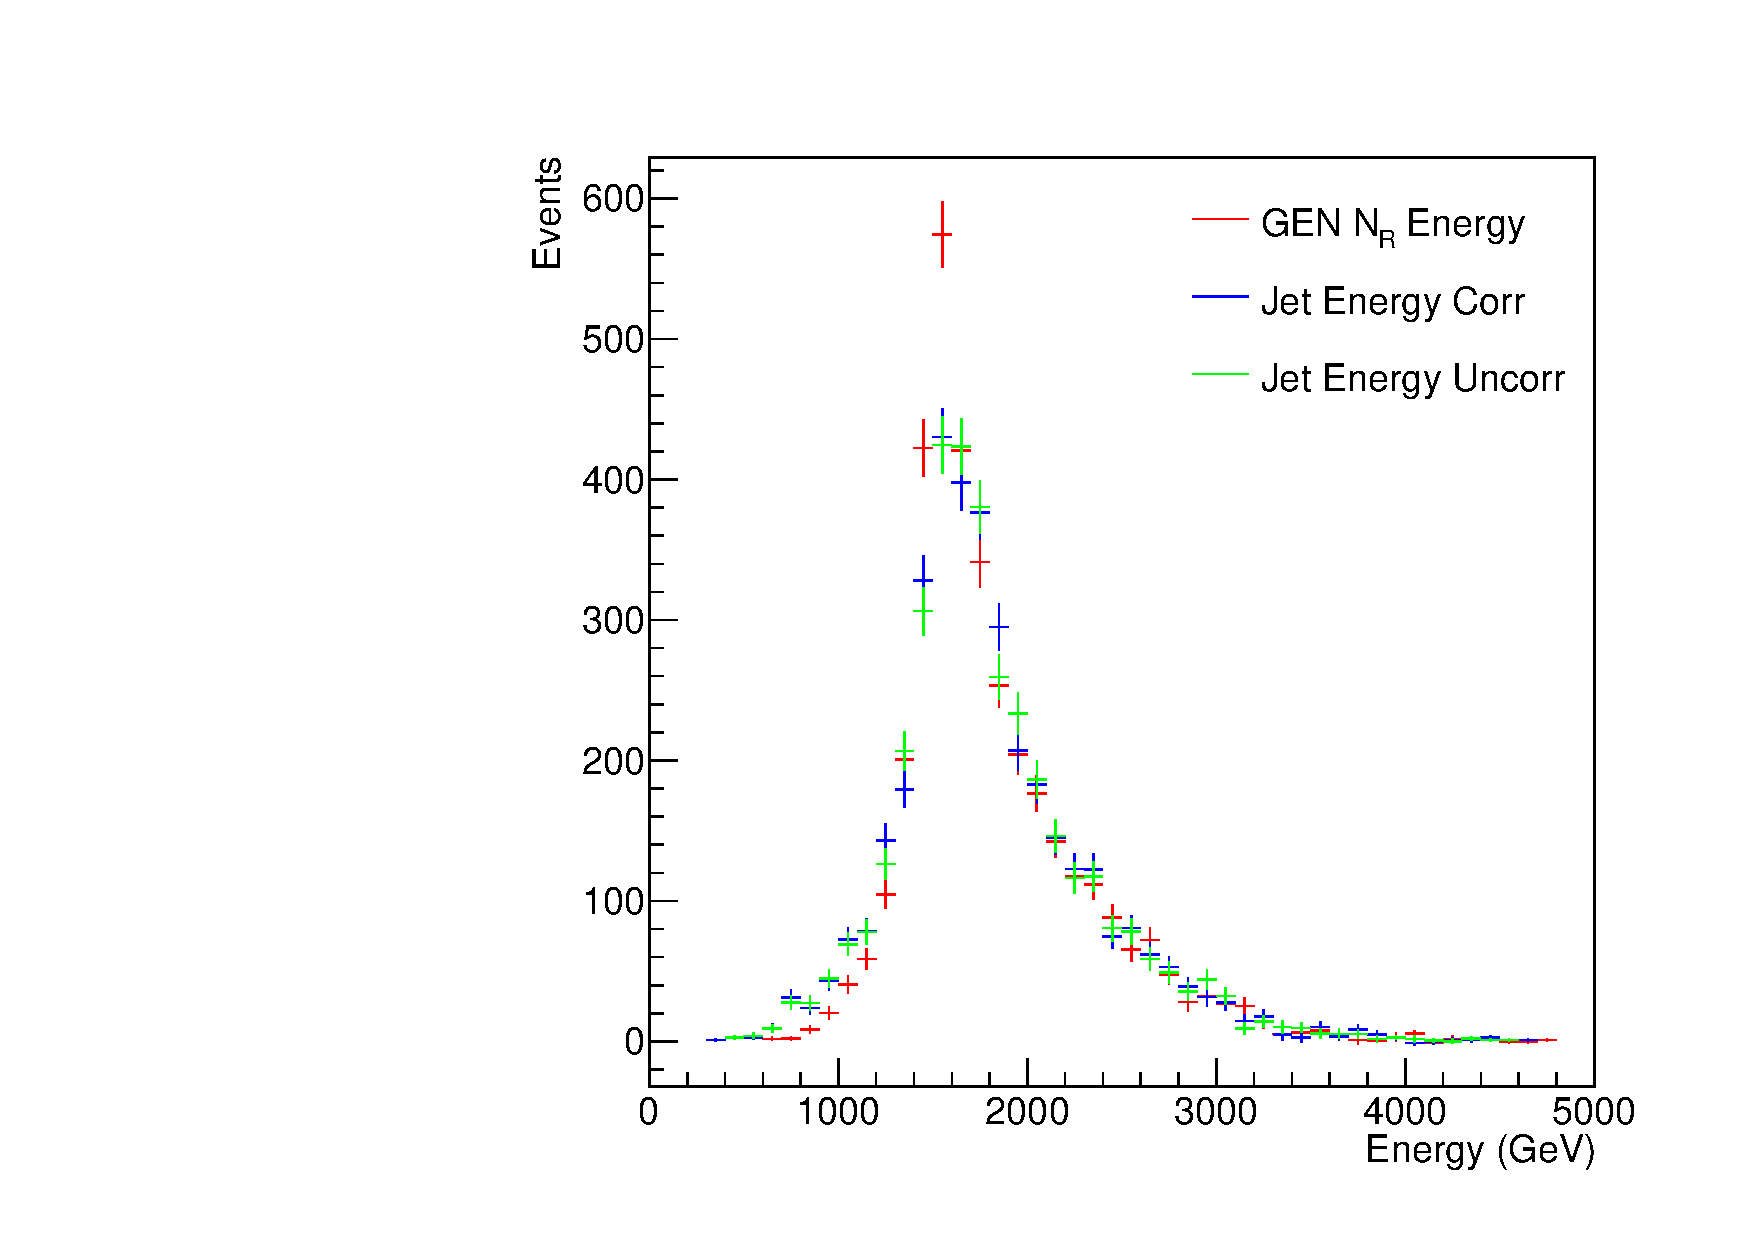
\includegraphics[width=\textwidth]{figures/JetEnergyVsNeutrinoEnergy_3000_400.pdf}
    \caption[
        %Short caption for the list of figures
       Reconstructed Jet Energy vs Generated Neutrino Energy.
    ]{
        % Full caption shown below the image
        The generated right-handed neutrino energy is compared to the corrected and uncorrected jet energy for the AK8 jet reconstructing the right-handed neutrino. 
    }
    % A label so you can \ref{fig:my_fig}. It is arbitrary; neither the 'fig:'
    % nor the fact that it has the same name as the pdf are required.
    \label{fig:jetEvsNRE}
\end{figure}

%\subsection{Soft-drop Jet Mass}
%In the boosted right-handed neutrino analysis case, the jet forming from the neutrino is expected to reconstruct with significant mass from a few hard constituents. With additional interactions occurring in the detector, the soft drop algorithm is used to mitigate wide-angle soft radiation in the jet contributing to its mass. Further information on the soft-drop algorithm can be seen in \ref{sec:softdrop}.

%\subsection{Lepton Subjet Fraction}
%The lepton subject fraction is calculated for each selected jet in the boosted analysis. The highest \pt momentum in the jet is used to calculated LSF for this jet. More on the LSF algorithm can be seen in \ref{sec:lsf},

\section{Muons}

\subsection{Reconstruction}
Muons in this analysis are required to be ``global''. Global muon reconstruction starts with hits recorded in the muon system and then looks for a matching track recorded in the tracker. There are several algorithms that perform this matching and more information on the muon reconstruction algorithms can be found in \cite{CMS-MUO-16-001}. Each algorithm is best suited for a specific range of muon $\eta$ and \pt values, so no single algorithm is always best for the high \pt muons studied in this analysis. This degeneracy in algorithm performance results from reductions in the tracker and muon detector momentum resolution as muon \pt increases. A specific combination of these algorithms, called \textsc{TuneP}, was chosen to determine the \pt of high energy muons. \textsc{TuneP} is used to recalculate all of the muons' \pt in this analysis.

\subsection{Identification}

Two types of muon identifications (ID) were used to select muons in this analysis. Isolated muons used in the resolved analysis, and the single isolated muon in the boosted analysis are all selected the same way. These are called ``high-$\pt$'' muons. The muon expected to be contained within the \NR jet is reconstructed with looser requirements as its reconstruction is expected to be more challenging. These are called ``loose'' muons. Loosening these requirements for this muon increases the acceptance rate of signal events without substantially increasing the background event rate.
The high-$\pt$ muon criteria are:
\begin{itemize}
\item The muon is reconstructed as a ``global'' muon.
\item At least one muon-chamber hit is included in the global-muon track fit.
\item There are muon segments in at least two muon stations.
\item The $\pt$ relative error, $\sigma_{\pt}/\pt$, of the muon best track, is less than 0.3.
\item To prevent muons from cosmic rays and from decays of long lived particles, the transverse impact parameter must be less than 2mm with respect to the primary vertex. The longitudinal distance of the track must be less than 5 mm from the primary vertex.
\item The muon track has at least one pixel hit.
\item At least 6 tracker layer hits are required in the reconstruction.
\end{itemize}
The Loose muon ID criteria are:
\begin{itemize}
\item The muon is a particle flow muon.
\item The muon is a ``global'' or ``tracker'' muon.
\end{itemize}

To reject muons from jets, each muon, other than the loose muon in boosted events, must be isolated from other tracks in the tracker. The energy of all tracks in a cone of $R = \sqrt{(\Delta\phi)^2 + (\Delta\eta)^2} < 0.3$ around the muon, excluding the muon track, must be less than 10\% of the muon $\pt$.
After applying these muon identification and isolation requirements, simulated events were re-weighted according to \CMS prescriptions to account for differences in the ID and isolation efficiencies between data and simulations~\cite{muonrochcorpaper, muonGEmethodpaper}.

%\subsection{Momentum Corrections}
%For muons with $\pt<200\GeV$, the momenta are corrected using the Rochester corrections~\cite{muonrochcorpaper}.
%Muons with $\pt\ge200\GeV$ are corrected with the generalized--endpoint (GE) method~\cite{muonGEmethodpaper}.
%These corrections bring the position and width of the \Ztomumu mass peak in simulations and data into better agreement.

\section{Electrons}
\label{sec:electron_reco}
\subsection{Reconstruction}
Electrons are reconstructed from \ECAL clusters matched to tracks made with the global-sum-fit (GSF) algorithm. The clusters in \ECAL are required to have a shower shape consistent with an electromagnetic interaction.
The energy measurement of electrons in \CMS is not perfect for various reasons. The measurements, however, can be corrected using the very precise measurement of the \Z boson mass from other experiments. \DYtoee events in \CMS are studied to generate these corrections. More details on the electron reconstruction can be found in \cite{particleFlow}\cite{electrons_8tev}.
%A scale factor is applied to electrons to correct for this mis-measurement according to the recipe provided by the Egamma POG.
Monte-Carlo events must also be corrected to account for differences between simulations and data in the energy resolution of electrons. Electrons in MC events are smeared to account for their artificially high resolution.
In total, electrons in MC are smeared, scaled, and the reconstruction efficiency is scaled based on the recommendations of the electron and photon (EGamma) POG~\cite{EGMsmearings, ELERECOSF, electrons_8tev}.

\subsection{Identification}
Reconstructed electrons are required to pass the high-energy electron-photon (HEEP) identification~\cite{HEEPID}.
This identification requires a reconstructed electron to contain a high quality, isolated track spatially linked to an isolated ECAL energy deposit.
In addition, the shower shape of the ECAL energy deposit must be consistent with a true electromagnetic shower. The requirements of HEEP are specifically tuned for high energy electrons, typically with $E > \SI{200}{\GeV}$.
The electrons have two selection categories (tight and loose), chosen such that resolved and boosted signal events are optimally reconstructed.
The ``Tight'' electron requirements are used to reconstruct both electrons for resolved events and the first electron in the boosted events.

Differences in electron ID efficiencies between data and simulation are taken into account by applying a scale factor provided by the EGamma POG~\cite{electrons_8tev}.
Discrepancies in energy scale and resolution between data and simulation are corrected following the EGamma POG prescriptions for scales and smearings~\cite{EGMsmearings}.
The electron energy scale was corrected in data, by a multiplicative factor dependent on both the $\eta$ and $R_{9}$ of the electron. Where $R_{9}$ is the ratio of the middle and surrounding $3\times3$ \ECAL crystals that the electron showers in.
The electron energy in simulated events was smeared to take into account the effective resolution in data. A Gaussian smearing which depends on $\eta$ and $R_{9}$ was applied.

The ``Loose'' electrons are used in boosted selection events to identify the electron lying within the AK8 jet. As the electron reconstruction is more challenging with the surrounding jet constituents, the electron identification requirements are loosened to keep signal acceptance high.
The requirements for electrons are summarized in Table~\ref{tab:ElectronSelection}.
\begin{table}[htb]


  \centering

  \begin{tabular}{ccc}
\hline
Requirement                     & Loose       & Tight \\
\hline
ID                                          & Cut Based Loose without relIsoWithEA & HEEPV70  \\
\hline
  
  \end{tabular}
   \caption[Electron selection requirements]{
    Electron selection requirements.
  }
\label{tab:ElectronSelection}
\end{table}

\section{HEM failure}
\label{sec:HEMfailure}
\CMS relies on particle flow to leverage information from as many sub-detectors as possible. As such, the loss of sectors in \HCAL as result of the HEM failure can be mitigated to some extent. The momentum and direction of particles can be determined from the tracker, as well as the sign of the charge.  Charged particles and photons interact in \ECAL and long-lived charged and neutral hadrons interact with \HCAL. Muon reconstruction typically relies on just the tracker and muon chambers, and are thus unaffected by the missing section of \HCAL.  Hadronic activity, however, suffers reduced precision as a unknown fraction of the hadronized particle's energy will be unmeasured. While the process of showering in the detector is relatively well understood, the amount of energy that would be expected in the dark region of \HCAL must be extrapolated. Electron identification also suffers. There are many different properties that distinguish electrons in the detector and one key way they are distinguished from charged pions is that charged pions shower in \ECAL and \HCAL. Electrons do not shower in \HCAL, as they are too light to penetrate this far.  The ratio of energy in \ECAL with the \HCAL sectors behind it is important to know, and impossible to extrapolate with \HCAL off.  
%Photons, on the other hand, are less affected, they offer up their entire energy in \ECAL and make a straight path through the tracker.  This makes them distinct from long lived neutral hadrons, which will shower in \HCAL and have no trace in the tracker.

To study the effects of the HEM failure on this analysis, the event rate in the low mass boosted signal region was studied. Both muon and electron flavor analyses were checked. The low mass signal region is the most similar selection to our actual signal region. Effects on this analysis were estimated to be related to the total number of events passing the analysis requirements as opposed to a change in reconstruction in the number of events. While it is probable that there is some level of effect from the HEM failure, as this analysis has very few events, any effect was determined to be smaller than the statistical precision available.

\begin{figure}[!tp]
\label{fig:hemfailure}
    \centering
    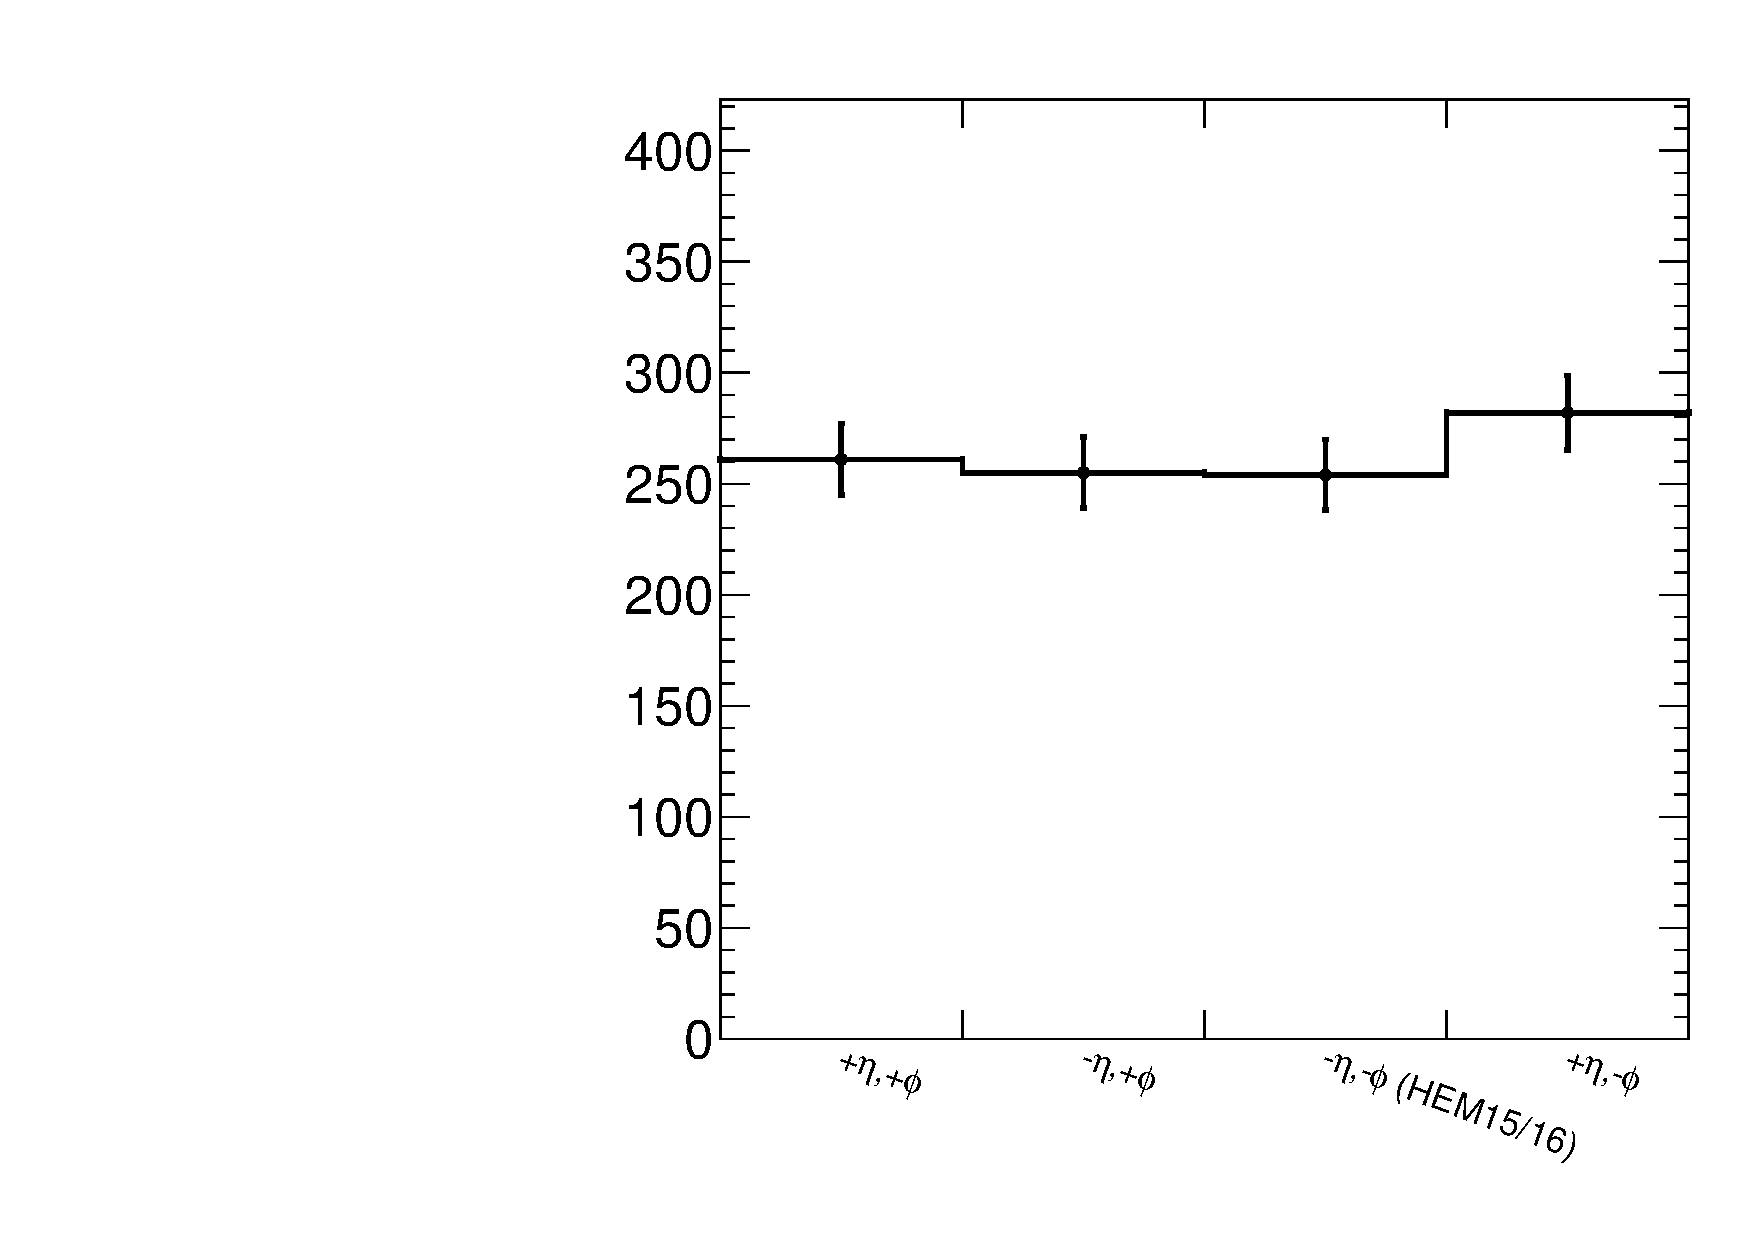
\includegraphics[width=0.49\textwidth]{figures/HEM1516/SingleMuon_AB_BoostedLowWRSR.pdf}
    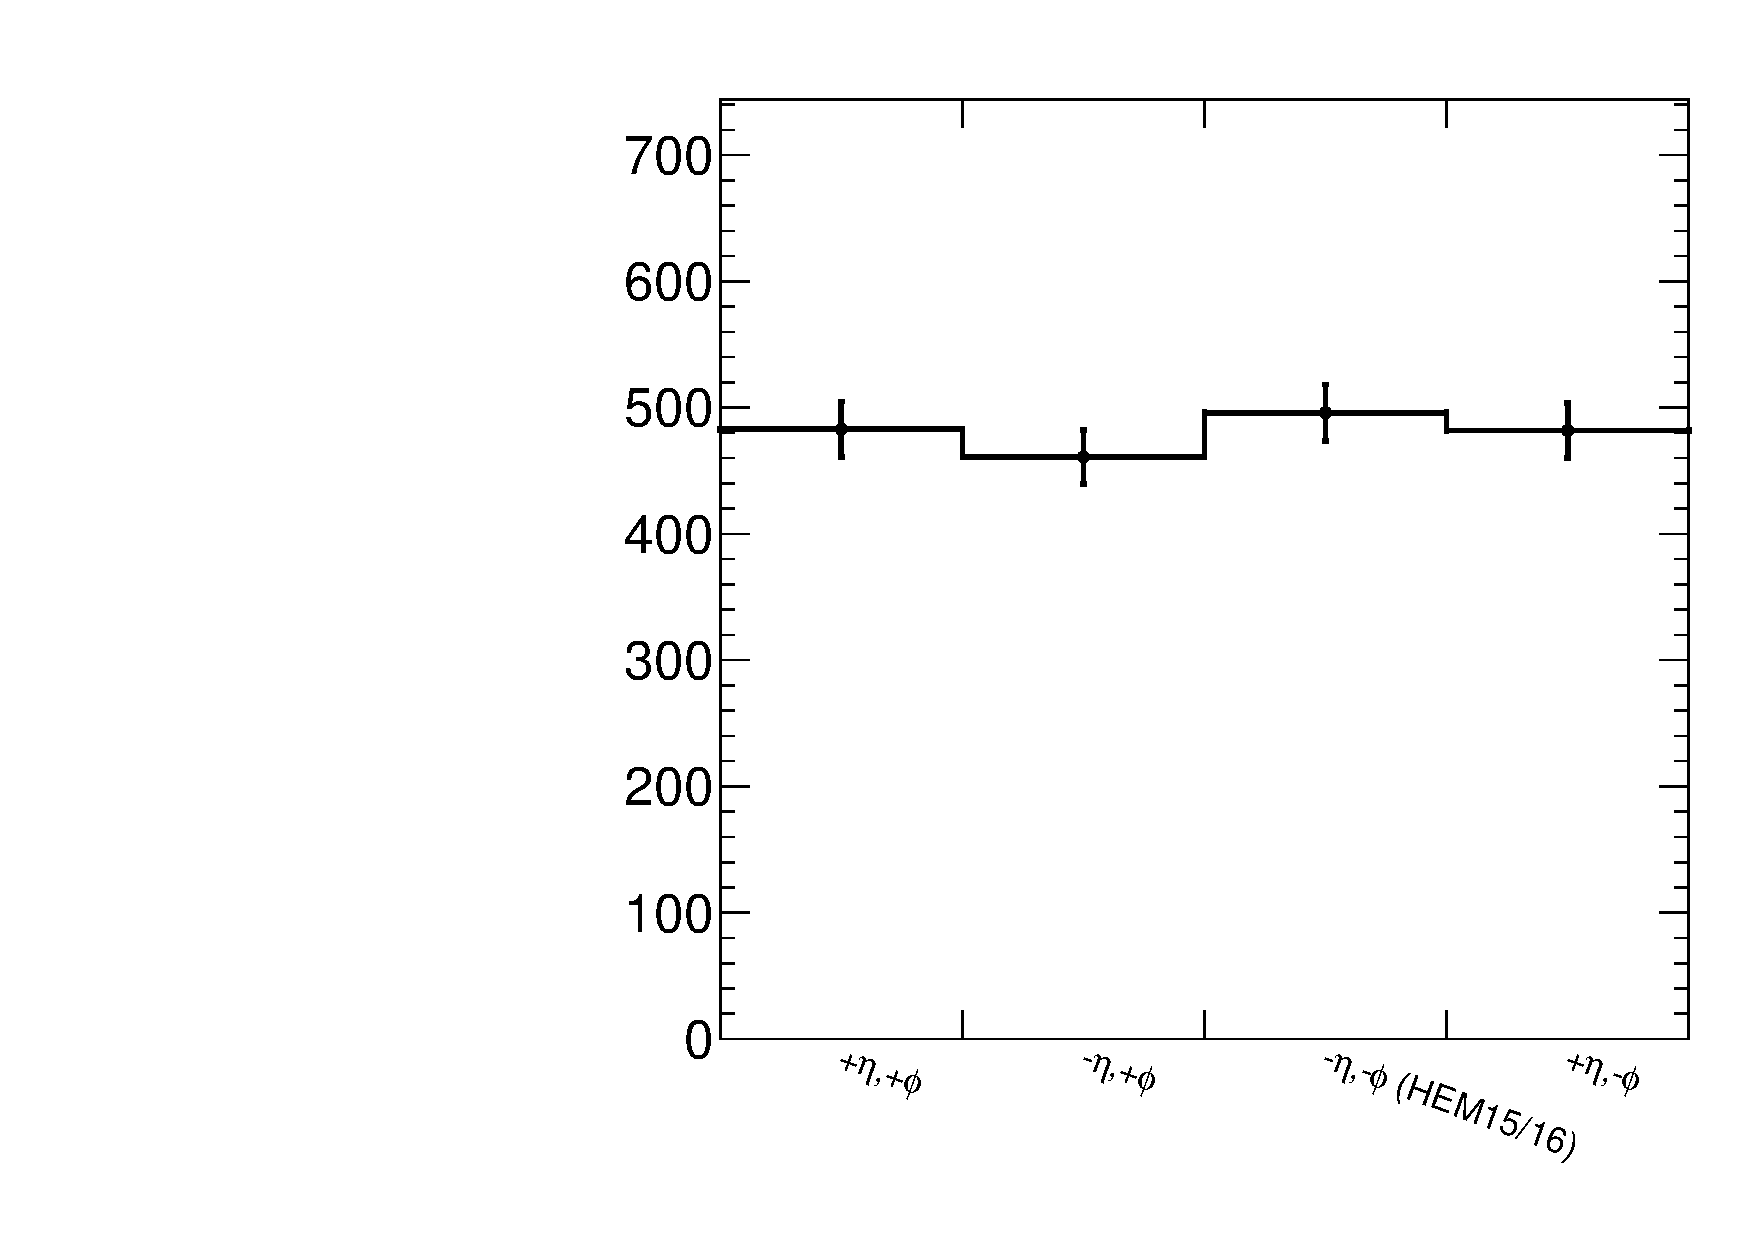
\includegraphics[width=0.49\textwidth]{figures/HEM1516/SingleMuon_CD_BoostedLowWRSR.pdf}
    \\
    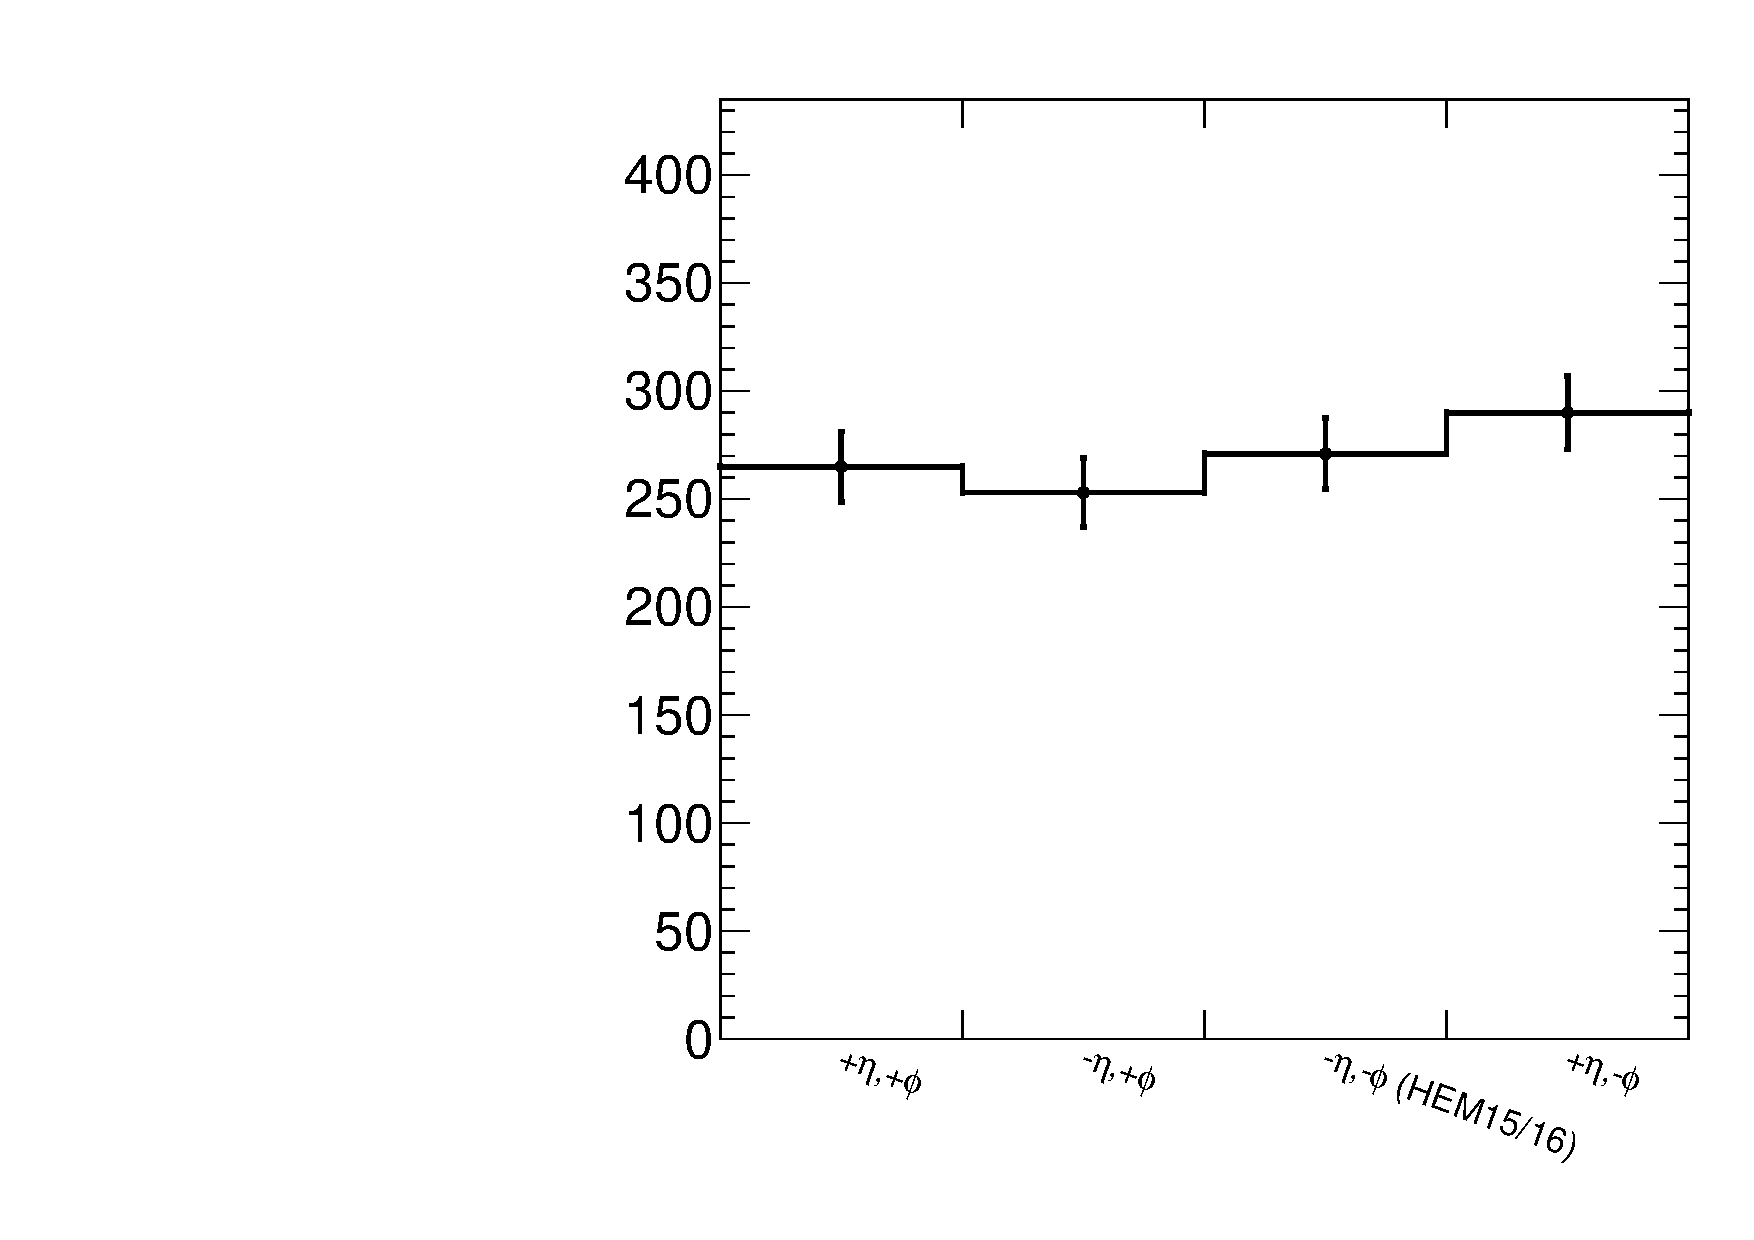
\includegraphics[width=0.49\textwidth]{figures/HEM1516/EGamma_AB_BoostedLowWRSR.pdf}
    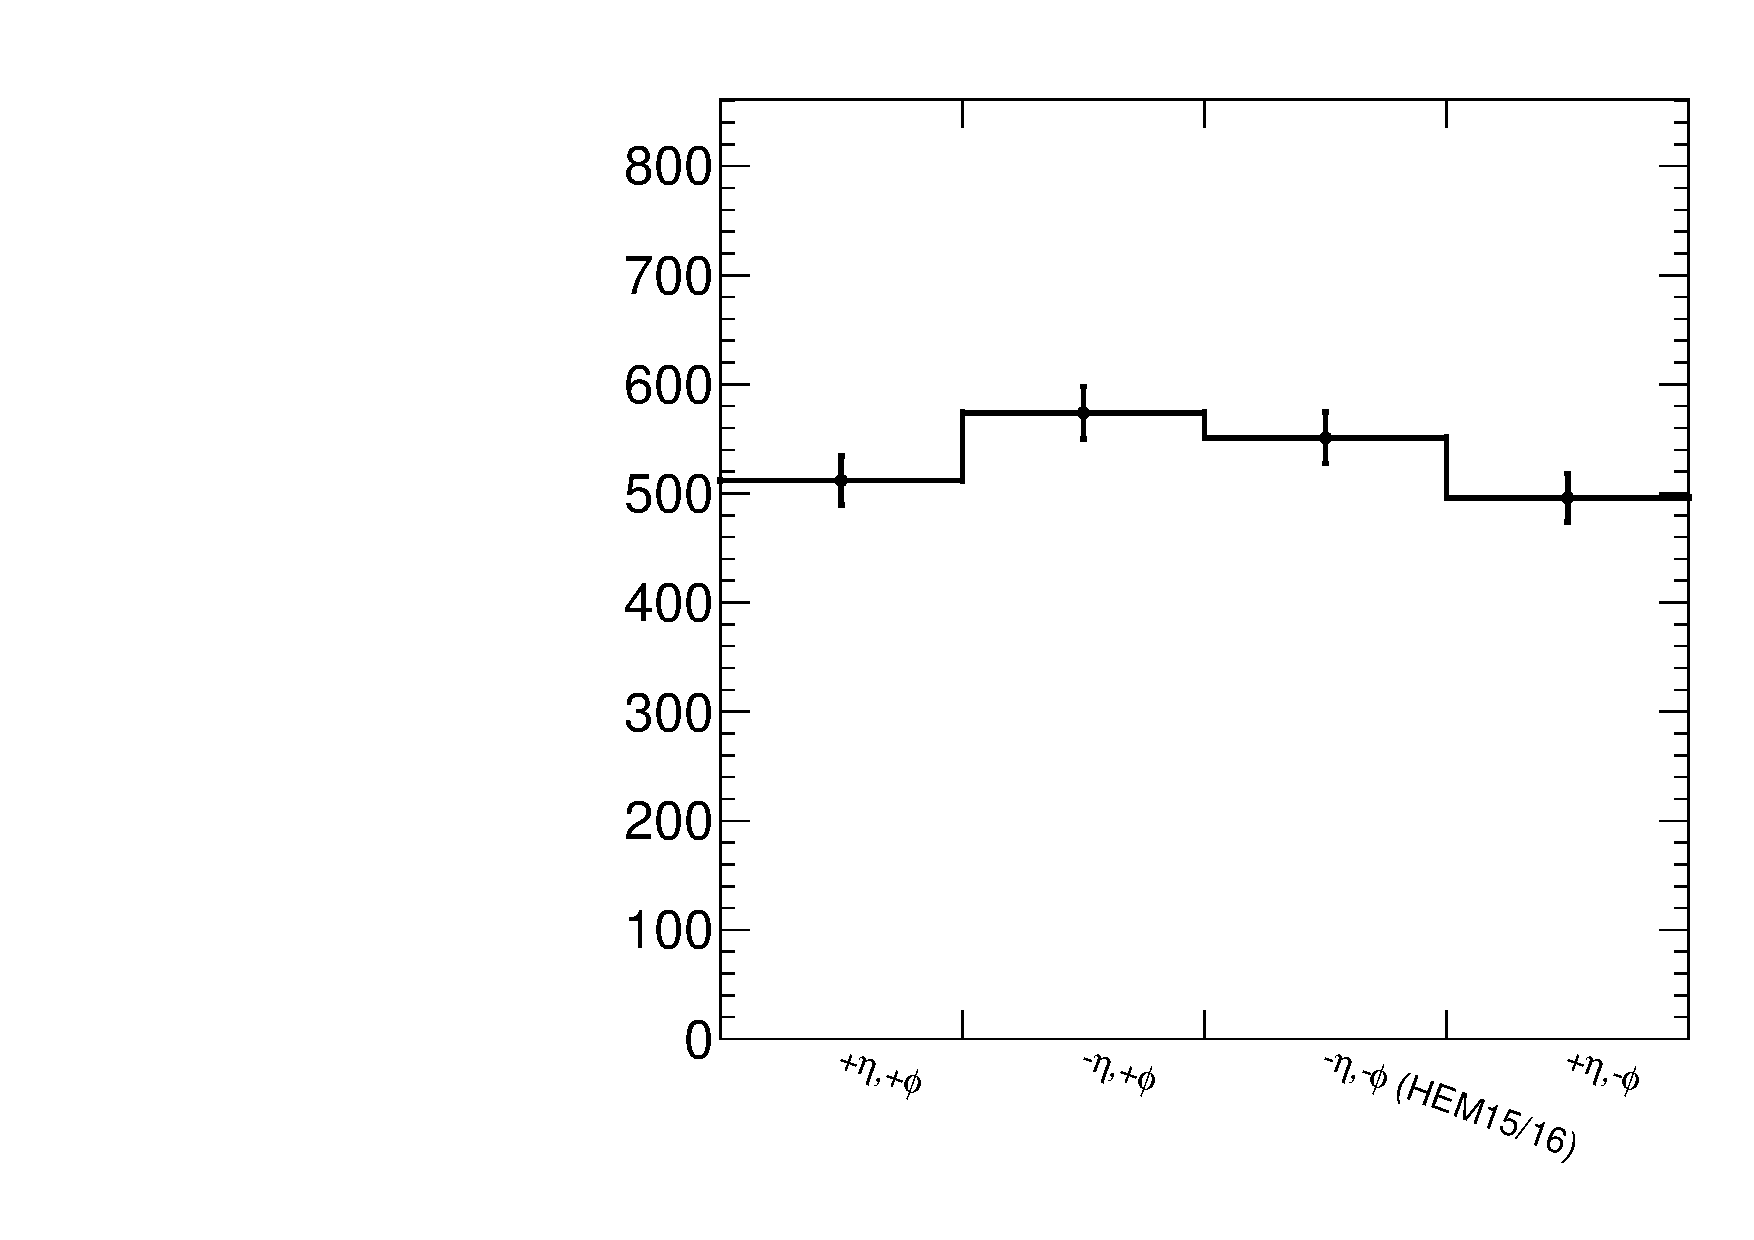
\includegraphics[width=0.49\textwidth]{figures/HEM1516/EGamma_CD_BoostedLowWRSR.pdf}
    
    \caption[
        %Short caption for the list of figures
       Event rate in the four complimentary quadrants of the endcap in eras of 2018.
    ]{
        % Full caption shown below the image
        The number of events passing the low mass signal selection with a particle within one of the four endcap quadrants is shown. In both rows, the data taking period prior to the the failure (eras A-B) are shown on the left. On the right, (eras C-D) rates of events after the failure are shown. The muon flavor analysis is on top and the electron flavor analysis is on bottom. In all of these regions the HEM failure region does not have a statistically significant difference.
    }
\end{figure}

\section{Triggers}
\label{sec:triggers}
The overarching goal of our trigger selection is simplicity. CMS defines hundreds of different requirement sets (triggers) to meet many needs. A trigger which only passes events with a very high muon \pt, for example, significantly reduces the amount of events needed to be sifted through.  Trigger selections must be careful not to be so strict as to reduce signal acceptance, while too-accepting triggers are overall problematic for the detector readout, as only so many events can be saved in a given amount of time.  Triggers accepting many events are generally pre-scaled.  Pre-scaling introduces a random selection designed to lower the rate at which a trigger passes events without biasing the trigger.

Trigger requirements can be thought of as coming in two forms. The first kind of requirement focuses on the quality of the object being triggered on. Requirements can be imposed to filter out objects that may come from detector noise, pileup, or are difficult to reconstruct for some reason (e.g. a muon that travels through a gap in the detector). These requirements lower the trigger rate and help ensure little of \CMS bandwidth is taken up by events that will eventually be rejected. On the other hand, these quality requirements will always reject ``good'' candidate objects at some rate and some quantity of truly interesting events will be lost to the bit bucket. 

Another sort of object requirement, like transverse momentum, does not directly require any object quality. However, high transverse momentum objects are reliable indicators of a particularly hard interaction in the detector. As the momentum requirement is raised, this requirement serves as an increasingly reliable proxy for object quality. As an example, the probability of a fake muon having several hundred GeV of momentum is extremely small. The advantage of a momentum trigger requirement is that as the momentum increases you can reasonably expect the efficiency to asymptotically approach the maximum possible value, given detector coverage.

A balance, then, is needed between object quality and transverse momentum. Thus, the path forward is to choose the most accepting triggers which are not yet so accepting to be pre-scaled.  Additional higher momentum (with less stringent identification) requiring triggers are then added to increase efficiency where a low momentum trigger may be lacking. This analysis uses single lepton triggers of corresponding flavor to the search region. Using a single lepton trigger is especially advantageous when multiple energetic leptons are expected in an event, as the combined probability of rejecting the event at the trigger level is much lower.
\subsection{Muon Triggers}
For simplicity, the boosted and resolved selection muon triggers are the same.  For each of the years the triggers are only slightly different.

\begin{table}[htbp]
  \caption[Muon Selection Triggers]{
    Muon Selection Triggers
  }
  \centering
  \label{tab:MuTrig}
  \begin{tabular}{cc}
\hline
Year & Triggers \\
\hline
2016 & \tt HLT\_Mu50\_v* OR HLT\_TkMu50\_v* \\
2017 & \tt HLT\_Mu50\_v* \\
2018 & \tt HLT\_Mu50\_v* OR HLT\_OldMu100\_v* OR HLT\_TK\_Mu100\_v* \\
\hline
  \end{tabular}
\end{table}

The HLT\_Mu50 triggers require a muon with at least \ensuremath{\SI{50}{\GeV}} to be in an event.  There were some inefficiencies with the detailed requirements of this trigger in 2016 and 2018, leading to the addition of triggers to complement the selection. Each of these selections are the recommended triggers specified by the muon physics object group (POG) at \CMS.

The trigger efficiencies used in our dimuon regions were officially measured by the muon POG as a function of the $\pt$ and $\eta$ of a muon passing the HighpT ID~\cite{MuonHLT2016, MuonHLT2017, MuonHLT2018}.
The efficiencies were measured in data and MC, and the ratio is used as a correction factor that is applied to MC.
The $\eta$ averaged $\pt$ behavior of these triggers in MC and data, as well as the ratio of data over MC can be seen in Figure~\ref{fig:MuonHLTweights}.

\begin{figure}[h!]\begin{center}
    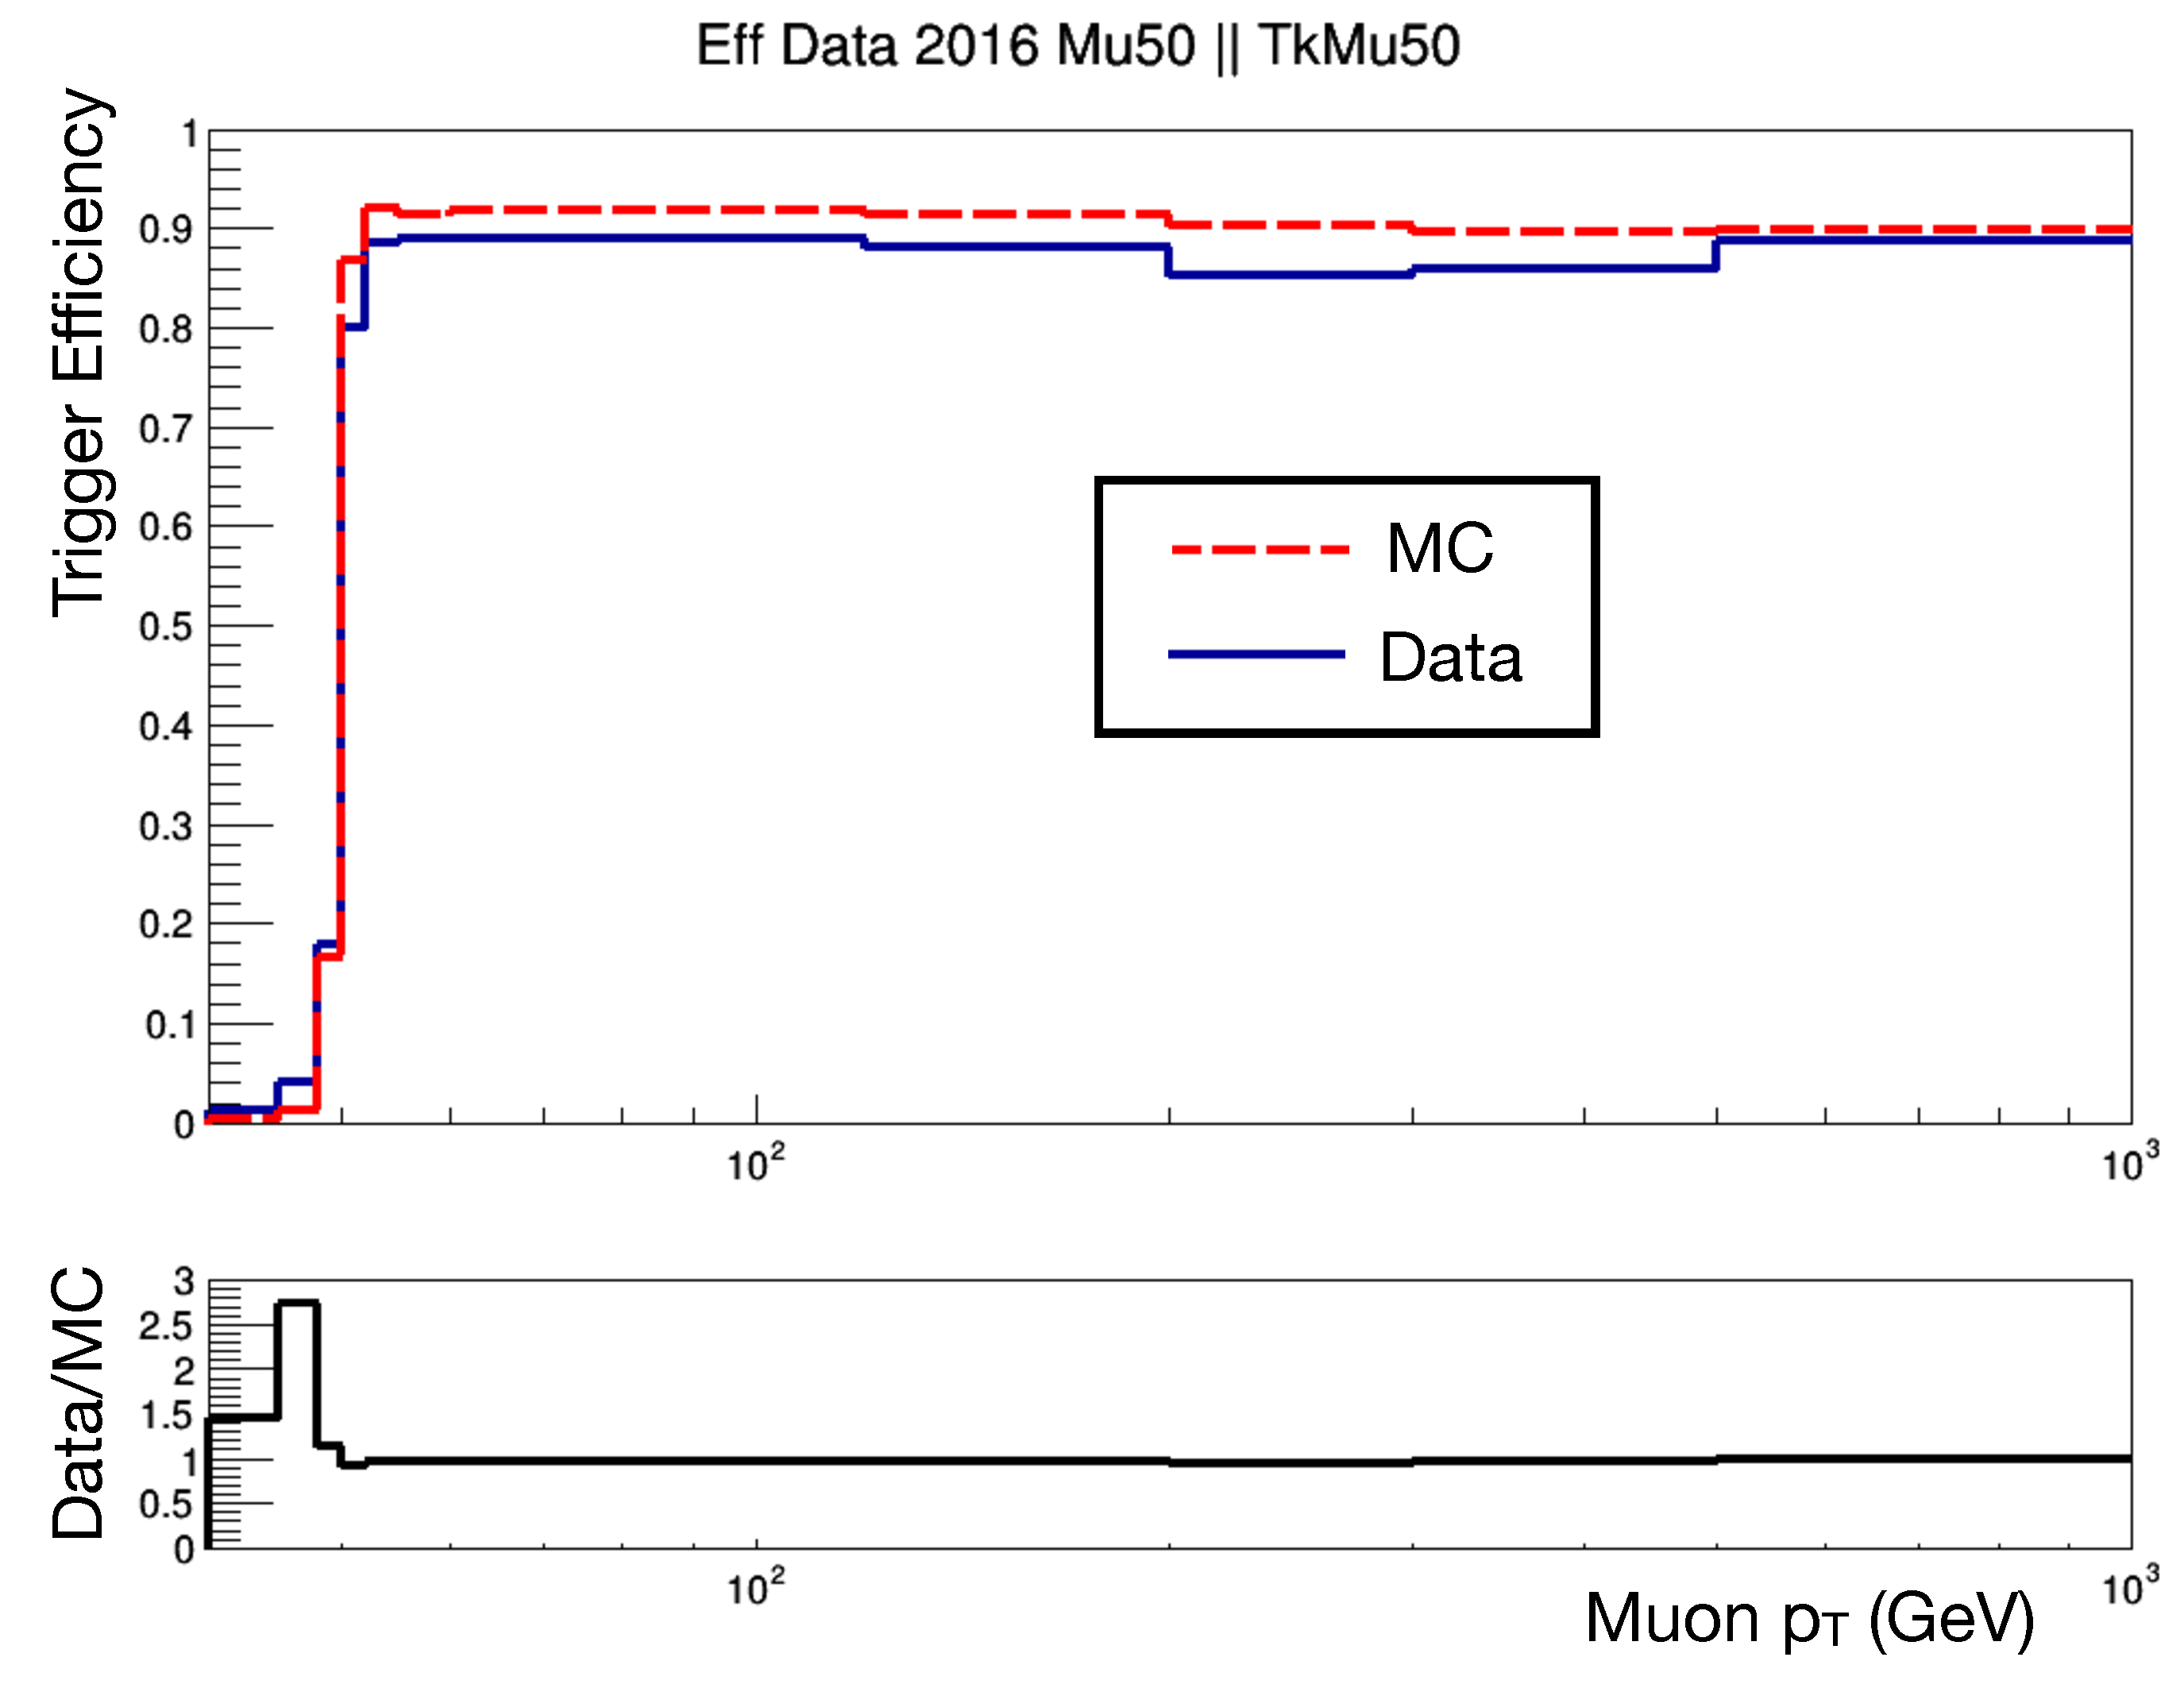
\includegraphics[width=0.49\textwidth]{figures/2016/SingleMuon/2016muonTrig.pdf}
    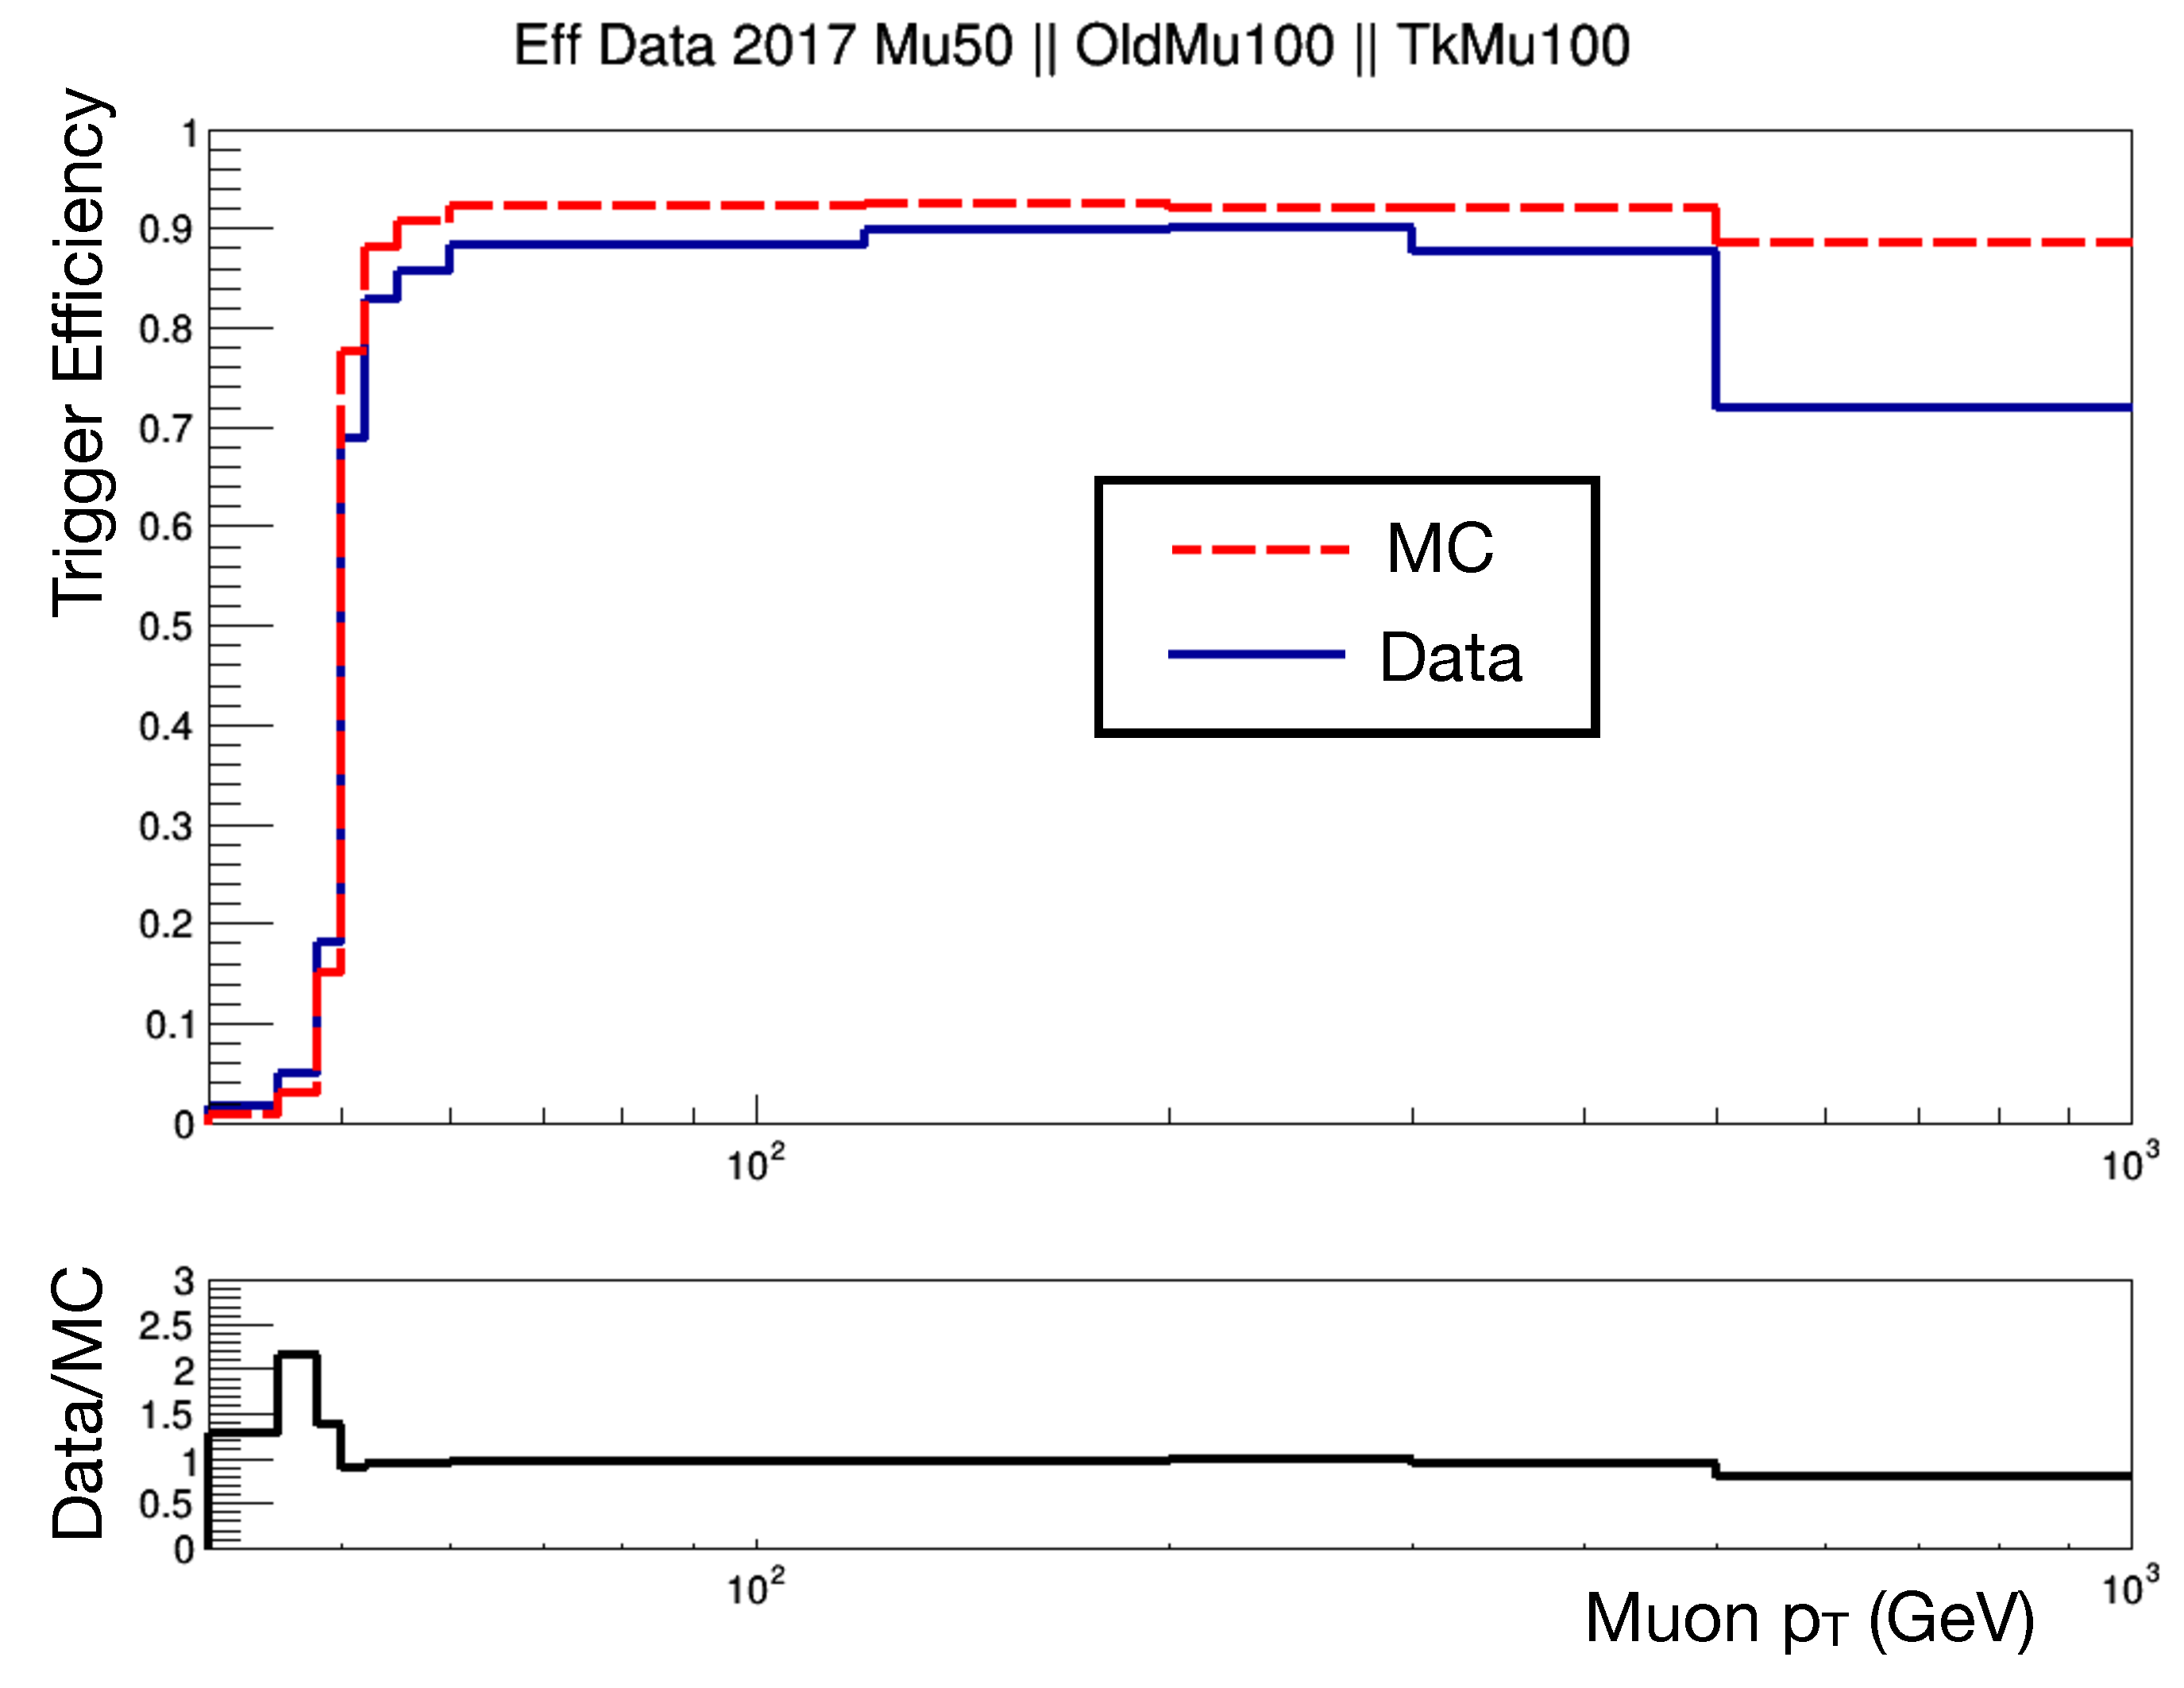
\includegraphics[width=0.49\textwidth]{figures/2017/SingleMuon/2017muonTrig.pdf}\\
    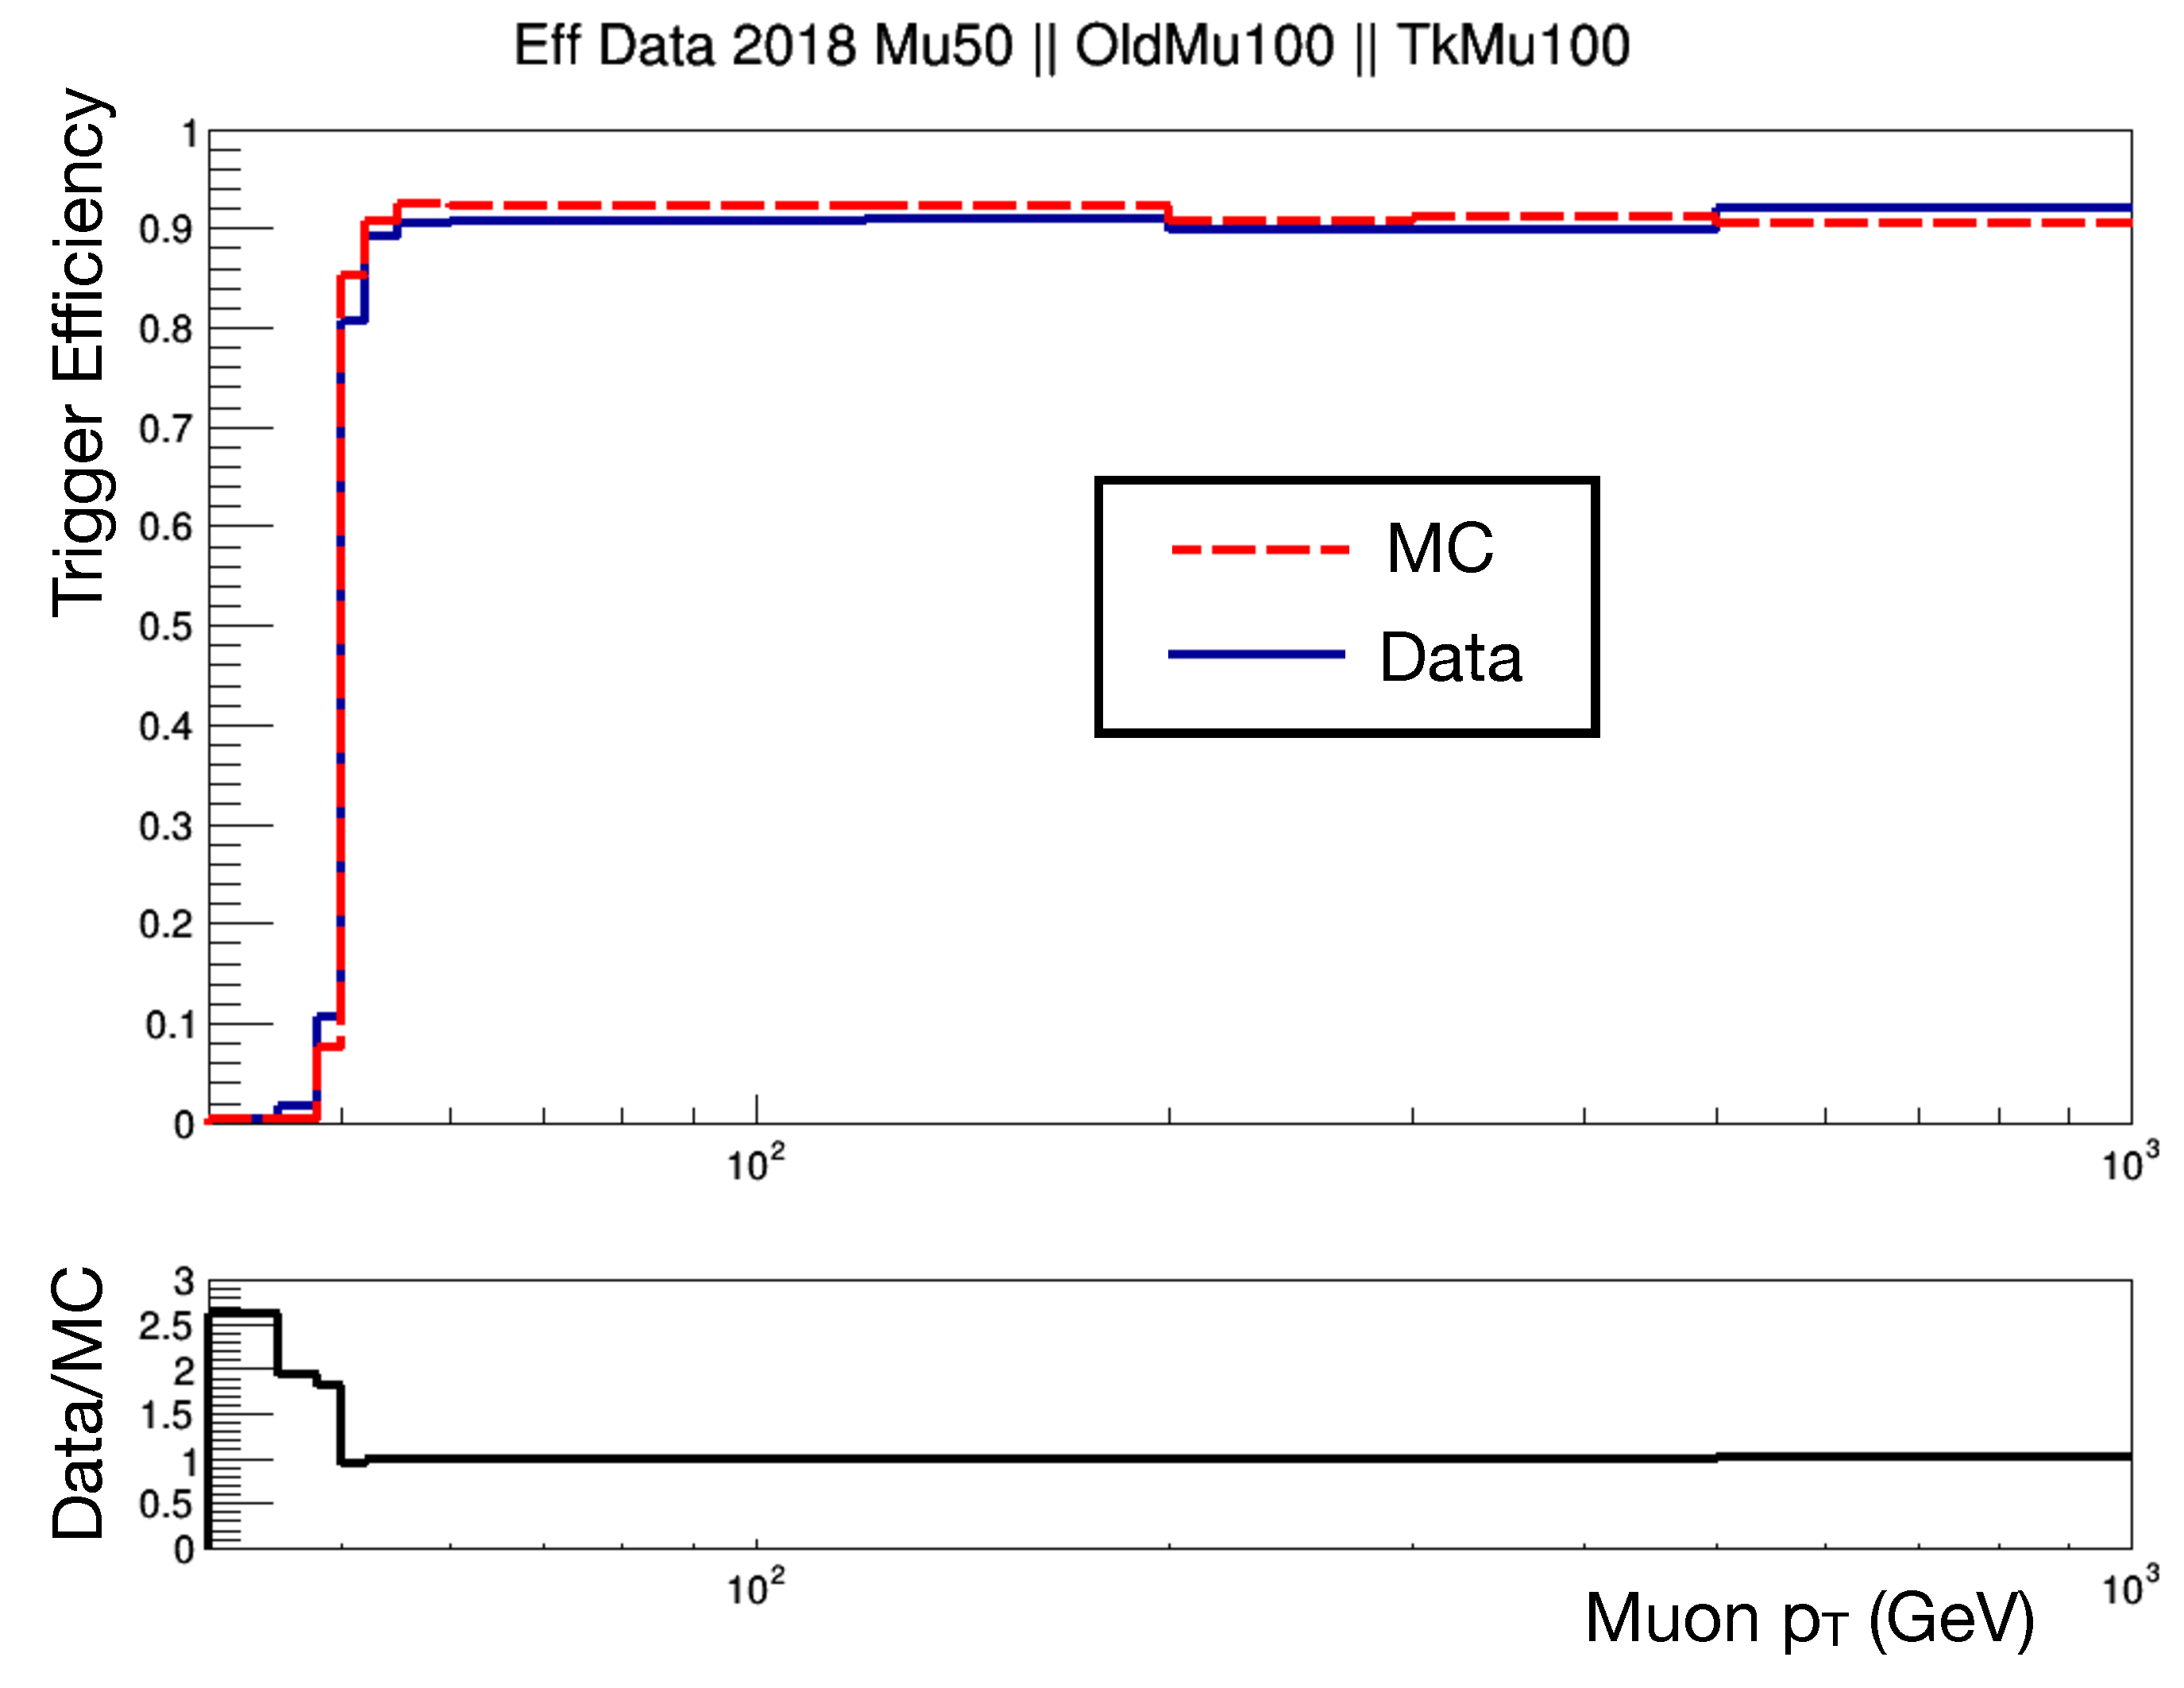
\includegraphics[width=0.49\textwidth]{figures/2018/2018muonTrig.pdf}
    
    \caption[Muon Trigger Efficiency]{Muon trigger efficiencies are shown for the 2016 (top left), 2017 (top right), and 2018 (bottom) years. The trigger combinations do rise quite high, but never become fully efficient at the highest muon momenta. Muon momenta becomes increasingly difficult to measure as higher $\pt$ as its path straightens in the detector.}
 \label{fig:MuonHLTweights}
 \end{center}
 \end{figure}

\subsection{Electron Triggers}
Electron trigger choice was more challenging than for muons. The lowest-$\pt$ threshold unprescaled trigger does not have as high an efficiency at higher $\pt$ as would be expected.  Two additional triggers were added, one higher $\pt$ electron trigger and one higher $\pt$ photon trigger. Electrons and photons can be differentiated later with parameters not used by the trigger. In addition, part of the 2017 data was not taken with the \texttt{HLT\_Ele115\_CaloIdVT\_GsfTrkIdT} trigger enabled, and so it is not included for the year. Omitting this trigger does make a small but distinguishable reduction in the overall trigger efficiency for a small mass region. 
Electrons falling in this region have less transverse momentum than a typical high $M_{\ell\ell jj}/M_{\ell J}$ event electron would have. 
As a result, the trigger change causes no perceptible change in the analysis performance.


\begin{table}[htbp]
  \caption[Electron Selection Triggers]{
    Electron Selection Triggers
  }
  \centering
  \label{tab:MuTrig}
  \begin{tabular}{l c}
    \hline
    Year & Trigger \\
    \hline
    2016 & \tt HLT\_Ele27\_WPTight\_Gsf\_v* OR HLT\_Ele115\_CaloIdVT\_GsfTrkIdT OR HLT\_Photon175\_v* \\
    2017 & \tt HLT\_Ele35\_WPTight\_Gsf\_v* OR HLT\_Photon200\_v* \\
    2018 & \tt HLT\_Ele32\_WPTight\_Gsf\_v* OR HLT\_Ele115\_CaloIdVT\_GsfTrkIdT OR HLT\_Photon200\_v* \\
    \hline
  \end{tabular}
\end{table}

\subsubsection{Electron Trigger Efficiencies}

The electron trigger combinations used in this analysis had not been officially studied.  As it is impossible to guarantee that the behaviour of a trigger applied to MC and data will be the same, all triggers, and trigger combinations, have to be studied.  The efficiency of the trigger combinations was measured in data and MC and compared to produce a scale factor as a function of electron $\pt$ and $\eta$.  Graphs showing the comparison of data and MC in each of the years are shown in Fig~\ref{fig:electronHLTSF}.  The $\eta$ dependence has to do with whether an electron lands in the barrel region or the endcap region and so these two regions are shown in black and red respectively.

\begin{figure}[htbp]
  \centering
  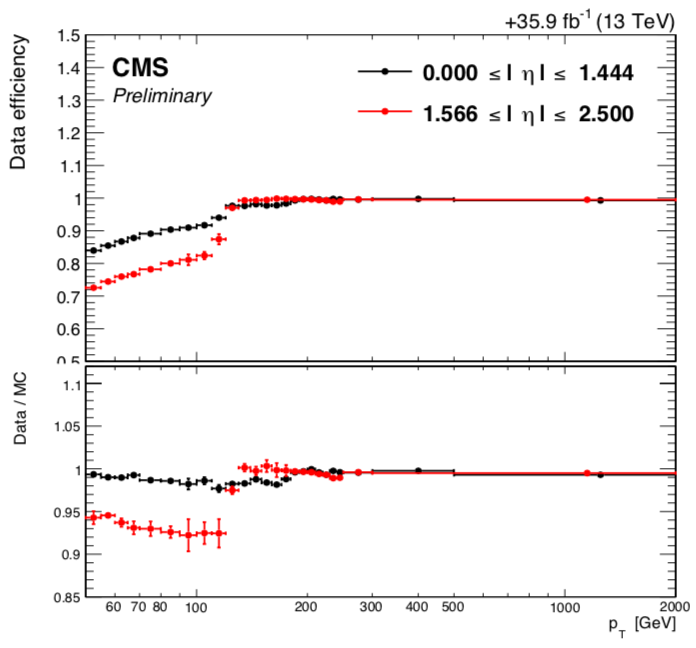
\includegraphics[width=0.45\textwidth]{figures/2016/2016_electron_HLT_SF.png}
  \vspace{0.01\textwidth}
  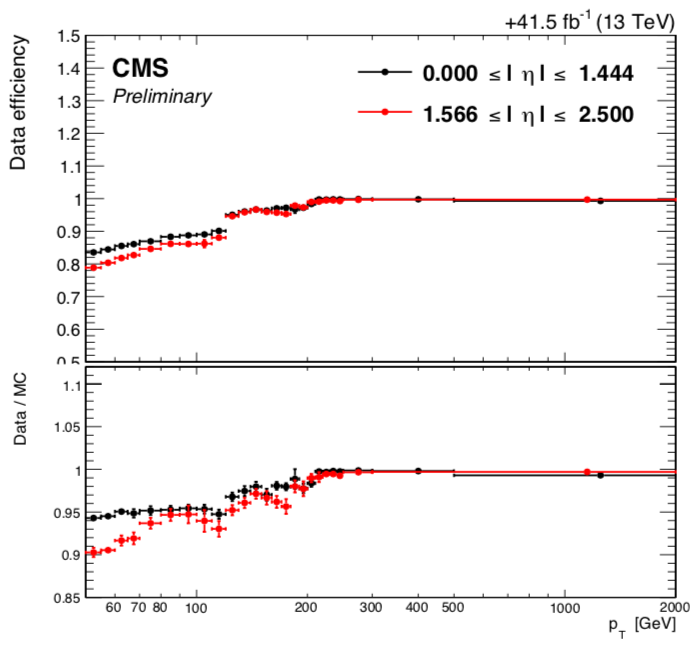
\includegraphics[width=0.45\textwidth]{figures/2017/2017_electron_HLT_SF.png}
  \vspace{0.01\textwidth}
  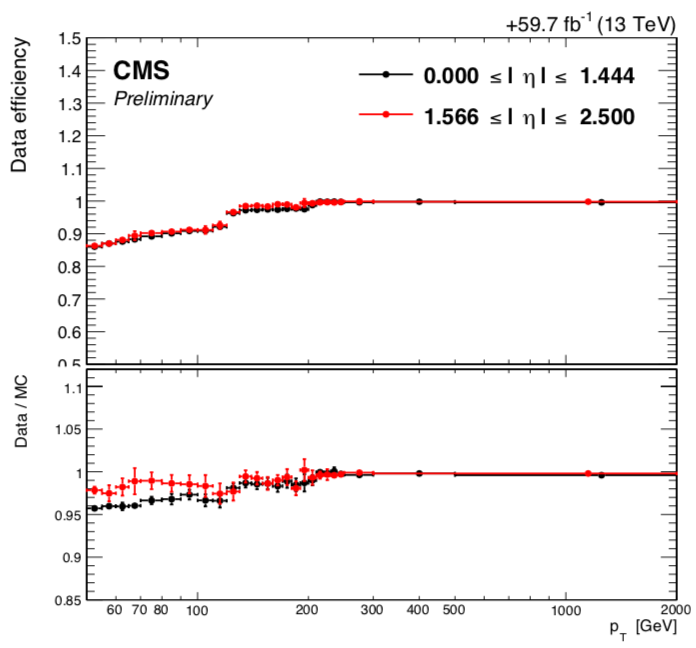
\includegraphics[width=0.45\textwidth]{figures/2018/2018_electron_HLT_SF.png}
  \caption[HLT Trigger Path Data-MC Comparison]{HLT trigger path comparison of data and MC.  Top left is 2016, 2017 is top right, and 2018 is on bottom.}
 
  \label{fig:electronHLTSF}
\end{figure}

\subsubsection{Level 1 Pre-Firing Trigger Inefficiency}

An issue with the \ECAL trigger system occurred during 2016 and 2017 due to the \ECAL trigger primitives. Information packaged by a subdetector and sent to the Level-1 (L1) trigger system are called trigger primitives.  These form the view of the \CMS detector at the L1 level.  In the inner-most rings of the \ECAL endcap, the timing of the detector began to drift, which increased the L1 pre-firing rate for all of the L1 triggers based on the calorimeters.

L1 pre-firing occurs when a L1 trigger fires based on the information from a trigger primitive (TP) which does not correspond to correct bunch crossing (BX).  The trigger primitive produced by \ECAL would have come from a certain BX, but because of a timing error, the BX prior to the trigger event is actually read out and sent to the HLT.  The \CMS trigger rules, which are designed to prevent buffer overflows vetoes more than one L1 trigger acceptance (L1A) signal in three consecutive BXs. The L1A from the incorrect BX then prevents the correct BX from being read out, even if it could have passed for other reasons.
A diagram of this is shown in Figure \ref{fig:L1prefire}.
\begin{figure}[!tp]
  \centering
  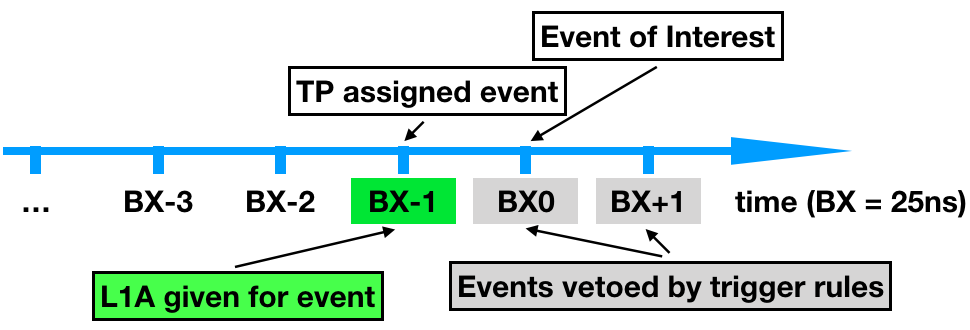
\includegraphics[width=\textwidth]{figures/prefire.png}
  \caption{The event of interest is shown as BX0.  Because of the timing shift, the TP is identified as being with BX-1, the L1A is issued for the wrong event, and the next two BXs are disallowed by trigger rules}
 
  \label{fig:L1prefire}
\end{figure}
While the timing drift causing the pre-firing is understood, there is no way to know on an event-by-event level if it occurred. There is, however, a way to guarantee that pre-firing did \emph{not} occur for a give event, by leveraging the trigger rules. Events which come only 3 BX after a previous L1A cannot be affected by the pre-firing issue. This is shown in Figure \ref{fig:L1unprefireable}.
\begin{figure}[!tp]
  \centering
  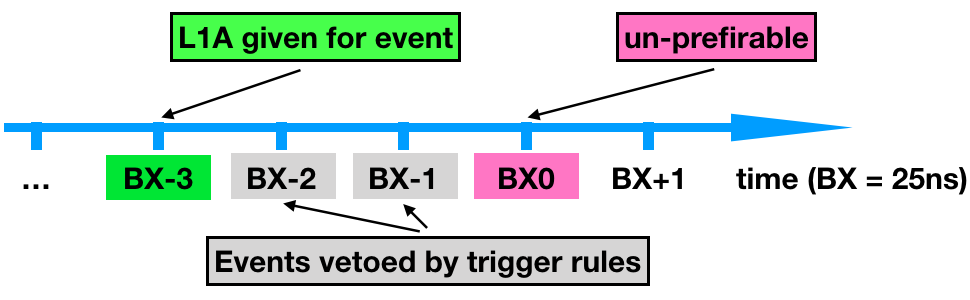
\includegraphics[width=\textwidth]{figures/unprefirable.png}
  \caption{The event of interest is shown as BX0.  Because of the trigger rules, if BX-3 has an L1A generated, BX-2, and BX-1 are ignored.  This means that BX0 cannot be affected by the pre-firing issue.}
 
  \label{fig:L1unprefireable}
\end{figure}

Each event that is saved records not just the L1 trigger information for the event, but also for the two BXs before and after. This means the probability that an L1 pre-fire could have occurred, if it were not for the trigger rules, can be calculated for these un-pre-fireable events. Using a tag-and-probe technique, the probability that an \ECAL interacting object could have its TP energy placed in the wrong BX can be calculated.  This effect must studied for every analysis done involving \ECAL. As each analysis will have different event requirements, the way the pre-firing issue affects it changes as well.

The pre-firing probabilities for this analysis are measured as a function of the $\pt$ and $\eta$ for jets, which deposit significant energy in \ECAL.  The events studied must have exactly one muon which corresponds to a passing decision from the HLT IsoMu24/27.  Electrons are vetoed.  The probed jet is required to pass tight identification requirements and be isolated with $\pt > \SI{40}{\GeV}$ as well as $1.75 < \abs{\eta} < 3.5$, placing it in the endcap, where pre-firing can happen.  The pre-firing probabilities for this are shown in Figure \ref{fig:prefireprobs}.
\begin{figure}[!tp]
  \centering
  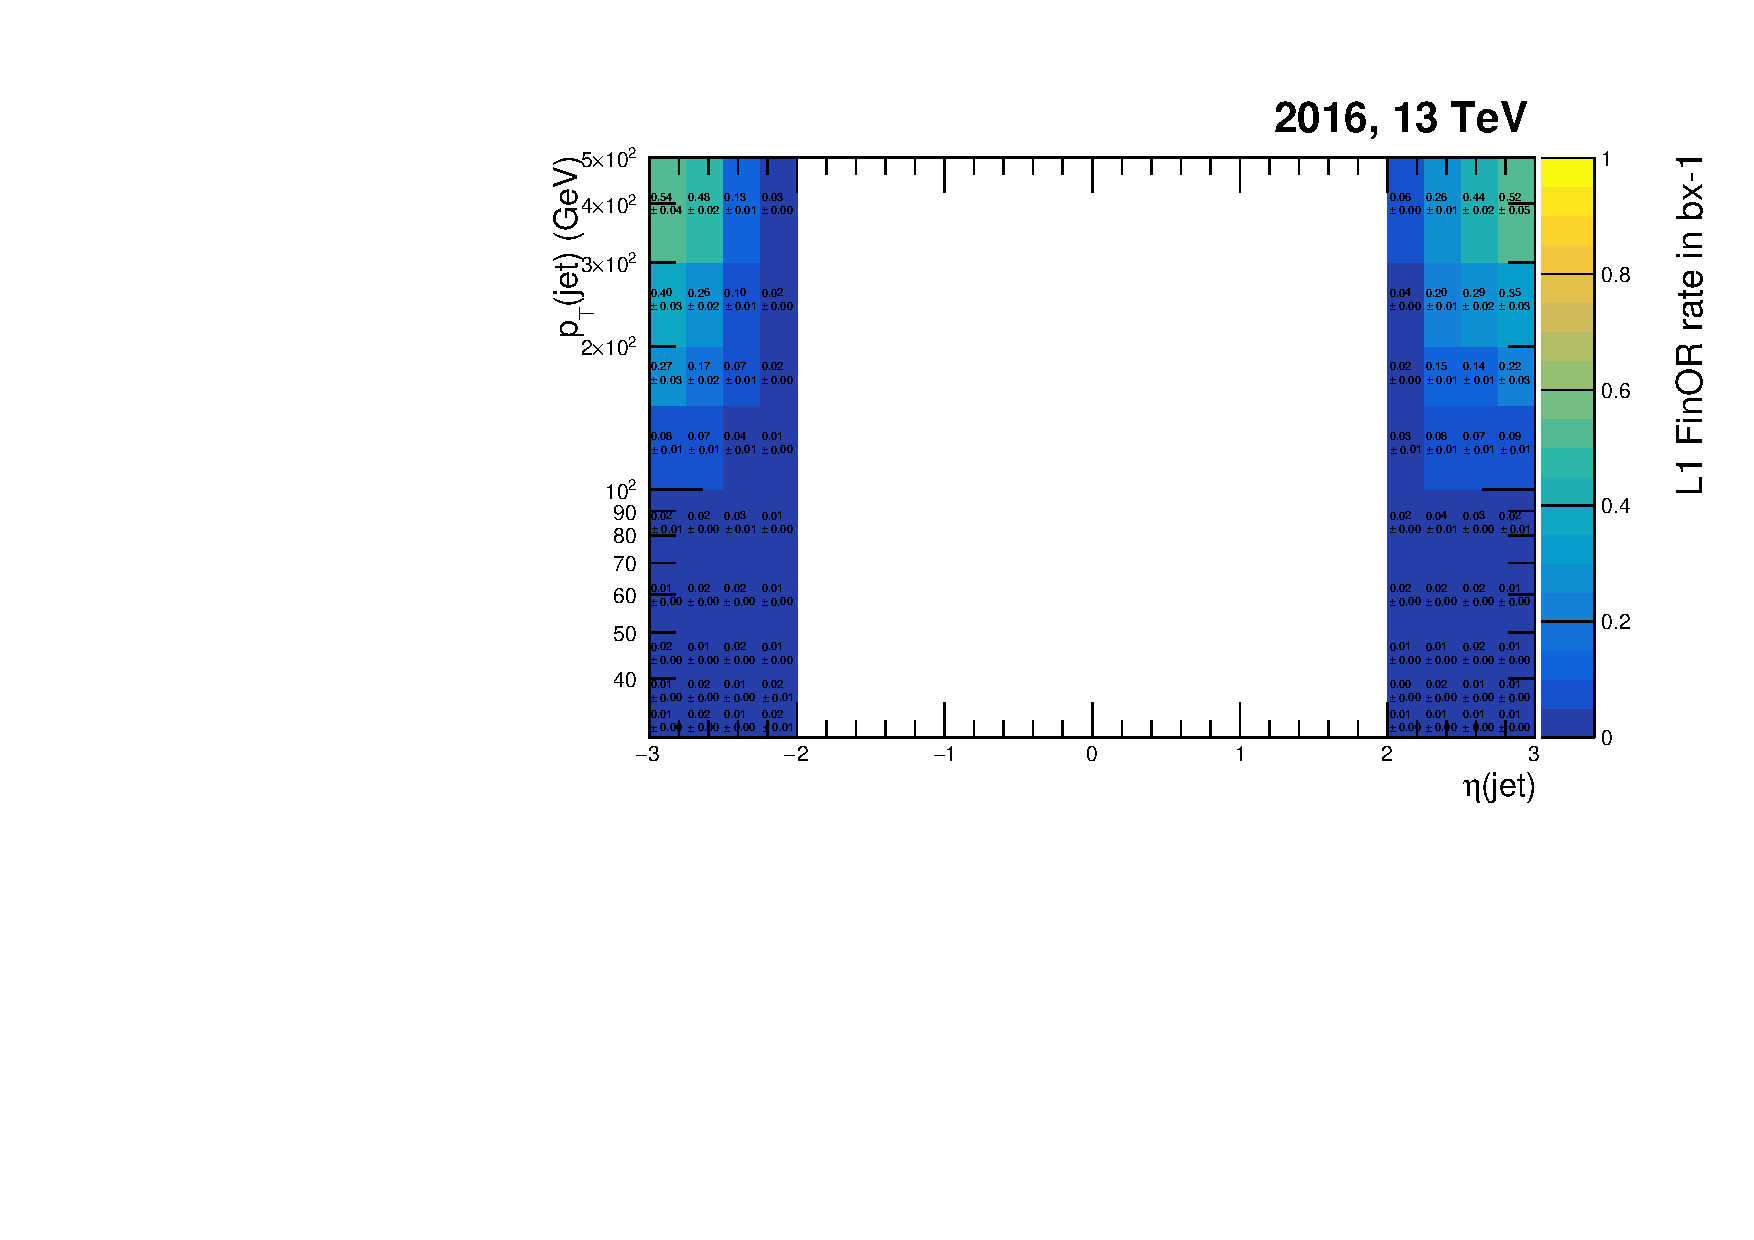
\includegraphics[width=0.45\textwidth]{figures/L1prefiring_jetpt_2016BtoH.pdf}
  \hspace{0.01\textwidth}
  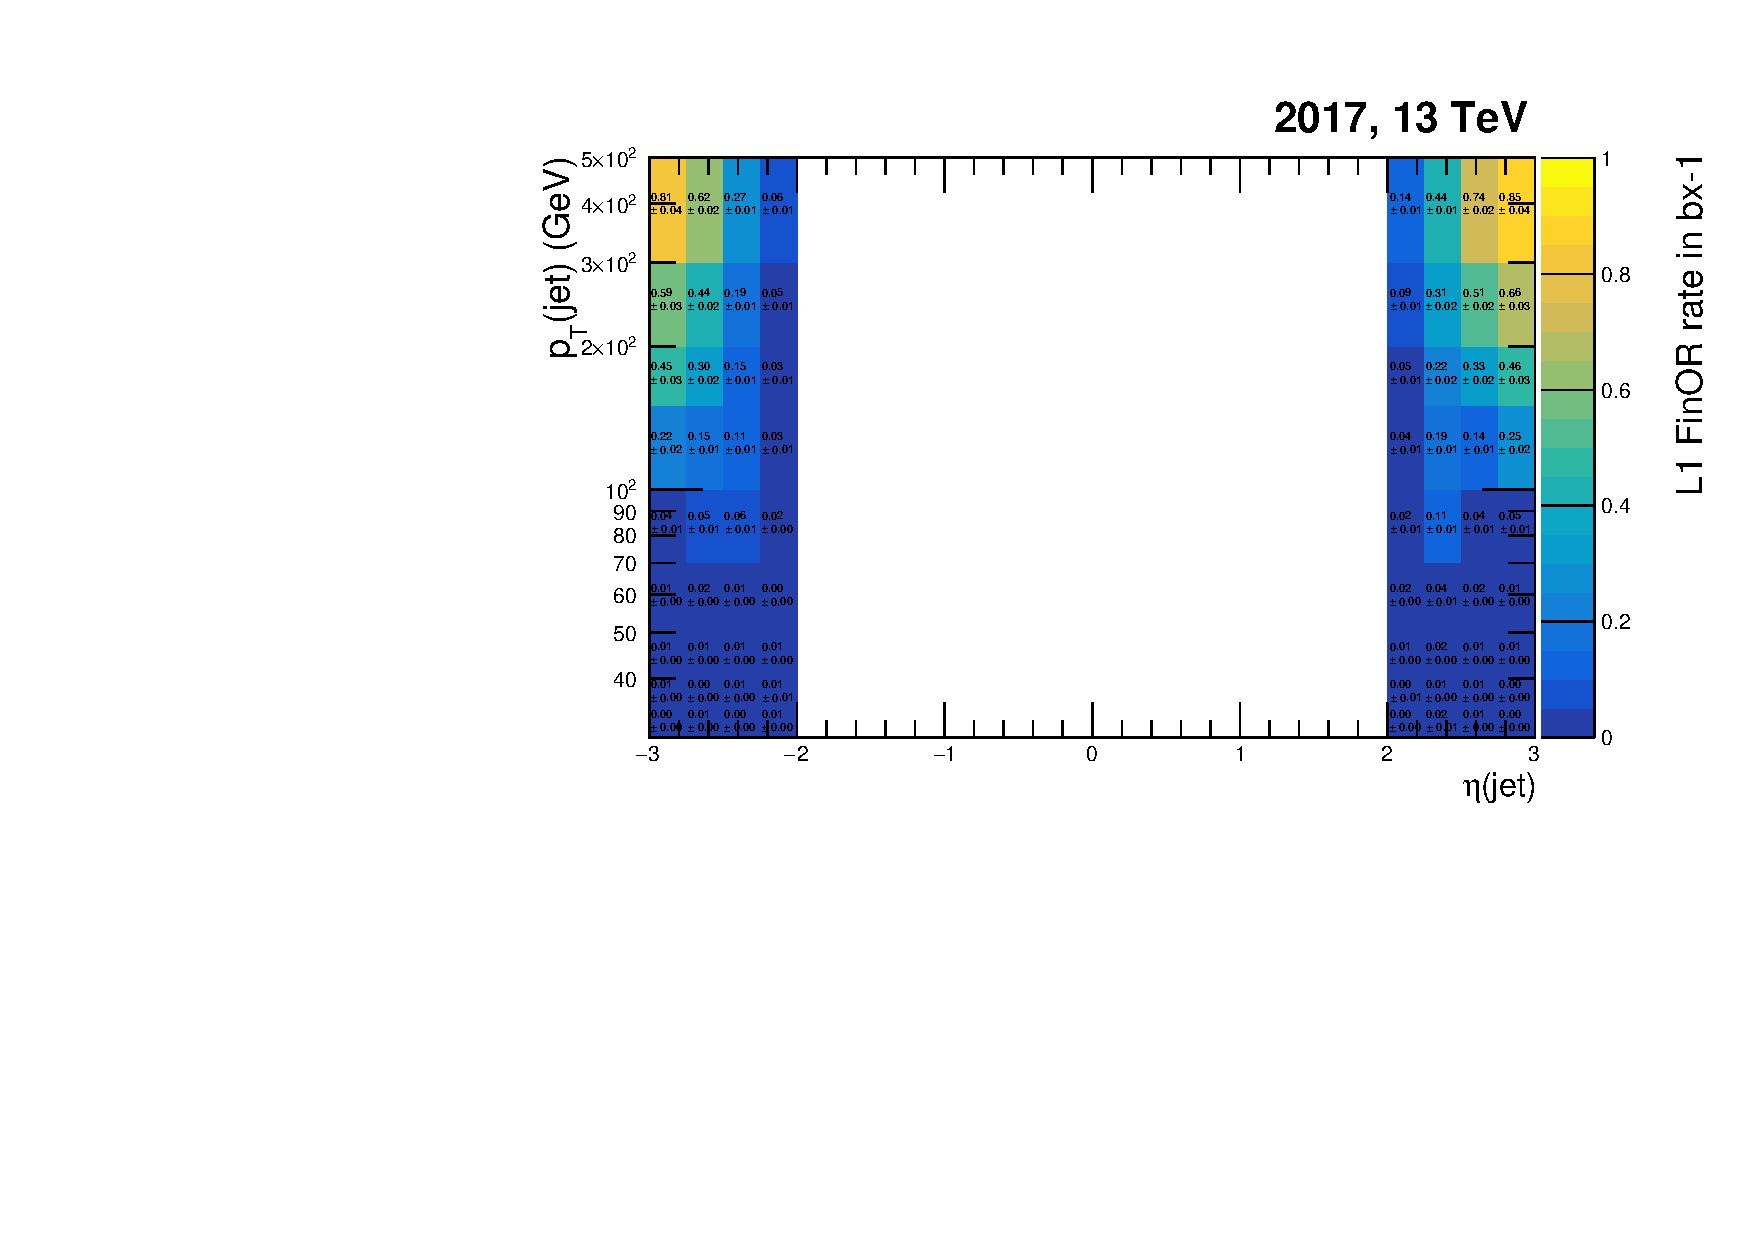
\includegraphics[width=0.45\textwidth]{figures/L1prefiring_jetpt_2017BtoF.pdf}
  \caption{The jet pre-firing probability for 2016 (left) and 2017 (right).}
  \label{fig:prefireprobs}
\end{figure}

These pre-firing probabilities are used to adjust the total jet rate in events taken in 2016 and 2017. As simulated events do not have the pre-firing issue, there is a mismatch of rates between data and MC.